% Generated by Sphinx.
\def\sphinxdocclass{report}
\documentclass[letterpaper,10pt,english]{sphinxmanual}
\usepackage[utf8]{inputenc}
\DeclareUnicodeCharacter{00A0}{\nobreakspace}
\usepackage{cmap}
\usepackage[T1]{fontenc}
\usepackage{babel}
\usepackage{times}
\usepackage[Bjarne]{fncychap}
\usepackage{longtable}
\usepackage{sphinx}
\usepackage{multirow}


\title{fantastico Documentation}
\date{June 05, 2013}
\release{0.1.0-b80}
\author{Radu Viorel Cosnita}
\newcommand{\sphinxlogo}{}
\renewcommand{\releasename}{Release}
\makeindex

\makeatletter
\def\PYG@reset{\let\PYG@it=\relax \let\PYG@bf=\relax%
    \let\PYG@ul=\relax \let\PYG@tc=\relax%
    \let\PYG@bc=\relax \let\PYG@ff=\relax}
\def\PYG@tok#1{\csname PYG@tok@#1\endcsname}
\def\PYG@toks#1+{\ifx\relax#1\empty\else%
    \PYG@tok{#1}\expandafter\PYG@toks\fi}
\def\PYG@do#1{\PYG@bc{\PYG@tc{\PYG@ul{%
    \PYG@it{\PYG@bf{\PYG@ff{#1}}}}}}}
\def\PYG#1#2{\PYG@reset\PYG@toks#1+\relax+\PYG@do{#2}}

\expandafter\def\csname PYG@tok@gd\endcsname{\def\PYG@tc##1{\textcolor[rgb]{0.63,0.00,0.00}{##1}}}
\expandafter\def\csname PYG@tok@gu\endcsname{\let\PYG@bf=\textbf\def\PYG@tc##1{\textcolor[rgb]{0.50,0.00,0.50}{##1}}}
\expandafter\def\csname PYG@tok@gt\endcsname{\def\PYG@tc##1{\textcolor[rgb]{0.00,0.27,0.87}{##1}}}
\expandafter\def\csname PYG@tok@gs\endcsname{\let\PYG@bf=\textbf}
\expandafter\def\csname PYG@tok@gr\endcsname{\def\PYG@tc##1{\textcolor[rgb]{1.00,0.00,0.00}{##1}}}
\expandafter\def\csname PYG@tok@cm\endcsname{\let\PYG@it=\textit\def\PYG@tc##1{\textcolor[rgb]{0.25,0.50,0.56}{##1}}}
\expandafter\def\csname PYG@tok@vg\endcsname{\def\PYG@tc##1{\textcolor[rgb]{0.73,0.38,0.84}{##1}}}
\expandafter\def\csname PYG@tok@m\endcsname{\def\PYG@tc##1{\textcolor[rgb]{0.13,0.50,0.31}{##1}}}
\expandafter\def\csname PYG@tok@mh\endcsname{\def\PYG@tc##1{\textcolor[rgb]{0.13,0.50,0.31}{##1}}}
\expandafter\def\csname PYG@tok@cs\endcsname{\def\PYG@tc##1{\textcolor[rgb]{0.25,0.50,0.56}{##1}}\def\PYG@bc##1{\setlength{\fboxsep}{0pt}\colorbox[rgb]{1.00,0.94,0.94}{\strut ##1}}}
\expandafter\def\csname PYG@tok@ge\endcsname{\let\PYG@it=\textit}
\expandafter\def\csname PYG@tok@vc\endcsname{\def\PYG@tc##1{\textcolor[rgb]{0.73,0.38,0.84}{##1}}}
\expandafter\def\csname PYG@tok@il\endcsname{\def\PYG@tc##1{\textcolor[rgb]{0.13,0.50,0.31}{##1}}}
\expandafter\def\csname PYG@tok@go\endcsname{\def\PYG@tc##1{\textcolor[rgb]{0.20,0.20,0.20}{##1}}}
\expandafter\def\csname PYG@tok@cp\endcsname{\def\PYG@tc##1{\textcolor[rgb]{0.00,0.44,0.13}{##1}}}
\expandafter\def\csname PYG@tok@gi\endcsname{\def\PYG@tc##1{\textcolor[rgb]{0.00,0.63,0.00}{##1}}}
\expandafter\def\csname PYG@tok@gh\endcsname{\let\PYG@bf=\textbf\def\PYG@tc##1{\textcolor[rgb]{0.00,0.00,0.50}{##1}}}
\expandafter\def\csname PYG@tok@ni\endcsname{\let\PYG@bf=\textbf\def\PYG@tc##1{\textcolor[rgb]{0.84,0.33,0.22}{##1}}}
\expandafter\def\csname PYG@tok@nl\endcsname{\let\PYG@bf=\textbf\def\PYG@tc##1{\textcolor[rgb]{0.00,0.13,0.44}{##1}}}
\expandafter\def\csname PYG@tok@nn\endcsname{\let\PYG@bf=\textbf\def\PYG@tc##1{\textcolor[rgb]{0.05,0.52,0.71}{##1}}}
\expandafter\def\csname PYG@tok@no\endcsname{\def\PYG@tc##1{\textcolor[rgb]{0.38,0.68,0.84}{##1}}}
\expandafter\def\csname PYG@tok@na\endcsname{\def\PYG@tc##1{\textcolor[rgb]{0.25,0.44,0.63}{##1}}}
\expandafter\def\csname PYG@tok@nb\endcsname{\def\PYG@tc##1{\textcolor[rgb]{0.00,0.44,0.13}{##1}}}
\expandafter\def\csname PYG@tok@nc\endcsname{\let\PYG@bf=\textbf\def\PYG@tc##1{\textcolor[rgb]{0.05,0.52,0.71}{##1}}}
\expandafter\def\csname PYG@tok@nd\endcsname{\let\PYG@bf=\textbf\def\PYG@tc##1{\textcolor[rgb]{0.33,0.33,0.33}{##1}}}
\expandafter\def\csname PYG@tok@ne\endcsname{\def\PYG@tc##1{\textcolor[rgb]{0.00,0.44,0.13}{##1}}}
\expandafter\def\csname PYG@tok@nf\endcsname{\def\PYG@tc##1{\textcolor[rgb]{0.02,0.16,0.49}{##1}}}
\expandafter\def\csname PYG@tok@si\endcsname{\let\PYG@it=\textit\def\PYG@tc##1{\textcolor[rgb]{0.44,0.63,0.82}{##1}}}
\expandafter\def\csname PYG@tok@s2\endcsname{\def\PYG@tc##1{\textcolor[rgb]{0.25,0.44,0.63}{##1}}}
\expandafter\def\csname PYG@tok@vi\endcsname{\def\PYG@tc##1{\textcolor[rgb]{0.73,0.38,0.84}{##1}}}
\expandafter\def\csname PYG@tok@nt\endcsname{\let\PYG@bf=\textbf\def\PYG@tc##1{\textcolor[rgb]{0.02,0.16,0.45}{##1}}}
\expandafter\def\csname PYG@tok@nv\endcsname{\def\PYG@tc##1{\textcolor[rgb]{0.73,0.38,0.84}{##1}}}
\expandafter\def\csname PYG@tok@s1\endcsname{\def\PYG@tc##1{\textcolor[rgb]{0.25,0.44,0.63}{##1}}}
\expandafter\def\csname PYG@tok@gp\endcsname{\let\PYG@bf=\textbf\def\PYG@tc##1{\textcolor[rgb]{0.78,0.36,0.04}{##1}}}
\expandafter\def\csname PYG@tok@sh\endcsname{\def\PYG@tc##1{\textcolor[rgb]{0.25,0.44,0.63}{##1}}}
\expandafter\def\csname PYG@tok@ow\endcsname{\let\PYG@bf=\textbf\def\PYG@tc##1{\textcolor[rgb]{0.00,0.44,0.13}{##1}}}
\expandafter\def\csname PYG@tok@sx\endcsname{\def\PYG@tc##1{\textcolor[rgb]{0.78,0.36,0.04}{##1}}}
\expandafter\def\csname PYG@tok@bp\endcsname{\def\PYG@tc##1{\textcolor[rgb]{0.00,0.44,0.13}{##1}}}
\expandafter\def\csname PYG@tok@c1\endcsname{\let\PYG@it=\textit\def\PYG@tc##1{\textcolor[rgb]{0.25,0.50,0.56}{##1}}}
\expandafter\def\csname PYG@tok@kc\endcsname{\let\PYG@bf=\textbf\def\PYG@tc##1{\textcolor[rgb]{0.00,0.44,0.13}{##1}}}
\expandafter\def\csname PYG@tok@c\endcsname{\let\PYG@it=\textit\def\PYG@tc##1{\textcolor[rgb]{0.25,0.50,0.56}{##1}}}
\expandafter\def\csname PYG@tok@mf\endcsname{\def\PYG@tc##1{\textcolor[rgb]{0.13,0.50,0.31}{##1}}}
\expandafter\def\csname PYG@tok@err\endcsname{\def\PYG@bc##1{\setlength{\fboxsep}{0pt}\fcolorbox[rgb]{1.00,0.00,0.00}{1,1,1}{\strut ##1}}}
\expandafter\def\csname PYG@tok@kd\endcsname{\let\PYG@bf=\textbf\def\PYG@tc##1{\textcolor[rgb]{0.00,0.44,0.13}{##1}}}
\expandafter\def\csname PYG@tok@ss\endcsname{\def\PYG@tc##1{\textcolor[rgb]{0.32,0.47,0.09}{##1}}}
\expandafter\def\csname PYG@tok@sr\endcsname{\def\PYG@tc##1{\textcolor[rgb]{0.14,0.33,0.53}{##1}}}
\expandafter\def\csname PYG@tok@mo\endcsname{\def\PYG@tc##1{\textcolor[rgb]{0.13,0.50,0.31}{##1}}}
\expandafter\def\csname PYG@tok@mi\endcsname{\def\PYG@tc##1{\textcolor[rgb]{0.13,0.50,0.31}{##1}}}
\expandafter\def\csname PYG@tok@kn\endcsname{\let\PYG@bf=\textbf\def\PYG@tc##1{\textcolor[rgb]{0.00,0.44,0.13}{##1}}}
\expandafter\def\csname PYG@tok@o\endcsname{\def\PYG@tc##1{\textcolor[rgb]{0.40,0.40,0.40}{##1}}}
\expandafter\def\csname PYG@tok@kr\endcsname{\let\PYG@bf=\textbf\def\PYG@tc##1{\textcolor[rgb]{0.00,0.44,0.13}{##1}}}
\expandafter\def\csname PYG@tok@s\endcsname{\def\PYG@tc##1{\textcolor[rgb]{0.25,0.44,0.63}{##1}}}
\expandafter\def\csname PYG@tok@kp\endcsname{\def\PYG@tc##1{\textcolor[rgb]{0.00,0.44,0.13}{##1}}}
\expandafter\def\csname PYG@tok@w\endcsname{\def\PYG@tc##1{\textcolor[rgb]{0.73,0.73,0.73}{##1}}}
\expandafter\def\csname PYG@tok@kt\endcsname{\def\PYG@tc##1{\textcolor[rgb]{0.56,0.13,0.00}{##1}}}
\expandafter\def\csname PYG@tok@sc\endcsname{\def\PYG@tc##1{\textcolor[rgb]{0.25,0.44,0.63}{##1}}}
\expandafter\def\csname PYG@tok@sb\endcsname{\def\PYG@tc##1{\textcolor[rgb]{0.25,0.44,0.63}{##1}}}
\expandafter\def\csname PYG@tok@k\endcsname{\let\PYG@bf=\textbf\def\PYG@tc##1{\textcolor[rgb]{0.00,0.44,0.13}{##1}}}
\expandafter\def\csname PYG@tok@se\endcsname{\let\PYG@bf=\textbf\def\PYG@tc##1{\textcolor[rgb]{0.25,0.44,0.63}{##1}}}
\expandafter\def\csname PYG@tok@sd\endcsname{\let\PYG@it=\textit\def\PYG@tc##1{\textcolor[rgb]{0.25,0.44,0.63}{##1}}}

\def\PYGZbs{\char`\\}
\def\PYGZus{\char`\_}
\def\PYGZob{\char`\{}
\def\PYGZcb{\char`\}}
\def\PYGZca{\char`\^}
\def\PYGZam{\char`\&}
\def\PYGZlt{\char`\<}
\def\PYGZgt{\char`\>}
\def\PYGZsh{\char`\#}
\def\PYGZpc{\char`\%}
\def\PYGZdl{\char`\$}
\def\PYGZhy{\char`\-}
\def\PYGZsq{\char`\'}
\def\PYGZdq{\char`\"}
\def\PYGZti{\char`\~}
% for compatibility with earlier versions
\def\PYGZat{@}
\def\PYGZlb{[}
\def\PYGZrb{]}
\makeatother

\begin{document}

\maketitle
\tableofcontents
\phantomsection\label{index::doc}



\chapter{Introduction}
\label{intro:introduction}\label{intro::doc}\label{intro:fantastico-framework}

\section{Why another python framework?}
\label{intro:why-another-python-framework}
The main reason for developing a new framework is simple: I want to use it for teaching purposes. I have seen many projects which
fail either because of poor coding or because they become legacy very fast. I will not get into details why and what could have
been done. It defeats the purpose.

Each piece of code that is being added to fantastico will follow these simple rules:
\begin{enumerate}
\item {} 
\emph{The code is written because is needed and there is no clean way to achieve the requirement with existing fantastico features}.

\item {} 
The code is developed using TDD (Test Driven Development).

\item {} 
The code quality is 9+ (reported by pylint).

\item {} 
The code coverage is 90\%+ (reported by nose coverage).

\item {} 
The code is fully documented and included into documentation.

\end{enumerate}


\subsection{What do you want to teach who?}
\label{intro:what-do-you-want-to-teach-who}
I am a big fan of Agile practices and currently I own a domain called scrum-expert.ro. This is meant to become a collection of
hands on resource of how to develop good software with high quality and in a reasonable amount of time. Resources will cover
topics like
\begin{enumerate}
\item {} 
Incremental development always ready for rollout.

\item {} 
TDD (Test Driven Development)

\item {} 
XP (eXtreme programming)

\item {} 
Scrum

\item {} 
Projects setup for Continuous Delivery

\end{enumerate}

and many other topics that are required for delivering high quality software but apparently so many companies are ignoring
nowadays.


\section{Fantastico's initial ideas}
\label{intro:fantastico-s-initial-ideas}\begin{itemize}
\item {} 
Very fast and pluggable routing engine.

\item {} 
Easily creation of REST apis.

\item {} 
Easily publishing of content (dynamic content).

\item {} 
Easily composition of available content.

\item {} 
Easily deployment on non expensive infrastructures (AWS, RackSpace).

\end{itemize}

Once the features above are developed there should be extremely easy to create the following sample applications:
\begin{enumerate}
\item {} 
Blog development

\item {} 
Web Forms development.

\item {} 
Personal web sites.

\end{enumerate}


\chapter{Getting started}
\label{get_started/getting_started:getting-started}\label{get_started/getting_started::doc}

\section{Installation manual}
\label{get_started/installation:installation-manual}\label{get_started/installation::doc}
In this section you can find out how to configure fantastico framework for different purposes.


\subsection{Developing a new fantastico project}
\label{get_started/installation:developing-a-new-fantastico-project}
Currently fantastico is in early stages so we did not really use it to create new projects. The desired way we want
to provide this is presented below:

pip-3.2 install fantastico

Done, now you are ready to follow our tutorials about creating new projects.


\subsection{Contributing to fantastico framework}
\label{get_started/installation:contributing-to-fantastico-framework}
Fantastico is an open source MIT licensed project to which any contribution is welcomed. If you like this framework idea
and you want to contribute do the following (I assume you are on an ubuntu machine):

\begin{Verbatim}[commandchars=\\\{\}]
\PYG{c}{\PYGZsh{}. Create a github account.}
\PYG{c}{\PYGZsh{}. Ask for permissions to contribute to this project (send an email to radu.cosnita@gmail.com) \PYGZhy{} I will gladly grant you permissions.}
\PYG{c}{\PYGZsh{}. Create a folder where you want to hold fantastico framework files. (e.g worspace\PYGZus{}fantastico)}
\PYG{c}{\PYGZsh{}. cd \PYGZti{}/workspace\PYGZus{}fantastico}
\PYG{c}{\PYGZsh{}. git clone git@github.com:rcosnita/fantastico}
\PYG{c}{\PYGZsh{}. sudo apt\PYGZhy{}get install python3\PYGZhy{}setuptools}
\PYG{c}{\PYGZsh{}. sh virtual\PYGZus{}env/setup\PYGZus{}dev\PYGZus{}env.sh}
\PYG{c}{\PYGZsh{}. cd \PYGZti{}/workspace\PYGZus{}fantastico}
\PYG{c}{\PYGZsh{}. git clone git@github.com:rcosnita/fantastico fantastico\PYGZhy{}doc}
\PYG{c}{\PYGZsh{}. git checkout gh\PYGZhy{}pages}
\end{Verbatim}

Now you have a fully functional fantastico workspace. I personally use PyDev and spring toolsuite but you are free to use
whatever editor you want. The only rule we follow is \emph{always keep the code stable}. To check the stability of your contribution
before commiting the code follow the steps below:

\begin{Verbatim}[commandchars=\\\{\}]
\PYG{c}{\PYGZsh{}. cd \PYGZti{}/workspace\PYGZus{}fantastico/fantastico/fantastico}
\PYG{c}{\PYGZsh{}. sh run\PYGZus{}tests.sh (we expect no failure in here)}
\PYG{c}{\PYGZsh{}. sh run\PYGZus{}pylint.sh (we expect 9+ rated code otherwise the build will fail).}
\PYG{c}{\PYGZsh{}. cd \PYGZti{}/workspace\PYGZus{}fantastico/fantastico}
\PYG{c}{\PYGZsh{}. export BUILD\PYGZus{}NUMBER=1}
\PYG{c}{\PYGZsh{}. ./build\PYGZus{}docs.sh (this will autogenerate documentation).}
\PYG{c}{\PYGZsh{}. Look into \PYGZti{}/workspace\PYGZus{}fantastico/fantastico\PYGZhy{}doc}
\PYG{c}{\PYGZsh{}. Here you can see the autogenerated documentation (do not commit this as Jenkins will do this for you).}
\PYG{c}{\PYGZsh{}. Be brave and push your newly awesome contribution.}
\end{Verbatim}


\section{Fantastico settings}
\label{get_started/settings:fantastico-settings}\label{get_started/settings::doc}
Fantastico is configured using a plain settings file. This file is located in the root of fantastico framework or in the root
folder of your project. Before we dig further into configuration options lets see a very simple settings file:

\begin{Verbatim}[commandchars=\\\{\}]
\PYG{k}{class} \PYG{n+nc}{BasicSettings}\PYG{p}{(}\PYG{n+nb}{object}\PYG{p}{)}\PYG{p}{:}
   \PYG{n+nd}{@property}
   \PYG{k}{def} \PYG{n+nf}{installed\PYGZus{}middleware}\PYG{p}{(}\PYG{n+nb+bp}{self}\PYG{p}{)}\PYG{p}{:}
      \PYG{k}{return} \PYG{p}{[}\PYG{l+s}{\PYGZdq{}}\PYG{l+s}{fantastico.middleware.request\PYGZus{}middleware.RequestMiddleware}\PYG{l+s}{\PYGZdq{}}\PYG{p}{,}
             \PYG{l+s}{\PYGZdq{}}\PYG{l+s}{fantastico.middleware.routing\PYGZus{}middleware.RoutingMiddleware}\PYG{l+s}{\PYGZdq{}}\PYG{p}{]}

   \PYG{n+nd}{@property}
   \PYG{k}{def} \PYG{n+nf}{supported\PYGZus{}languages}\PYG{p}{(}\PYG{n+nb+bp}{self}\PYG{p}{)}\PYG{p}{:}
      \PYG{k}{return} \PYG{p}{[}\PYG{l+s}{\PYGZdq{}}\PYG{l+s}{en\PYGZus{}us}\PYG{l+s}{\PYGZdq{}}\PYG{p}{]}
\end{Verbatim}

The above code sample represent the minimum required configuration for fantastico framework to run. The order in which middlewares
are listed is the order in which they are executed when an http request is made.


\subsection{Settings API}
\label{get_started/settings:settings-api}
Below you can find technical information about settings.
\index{BasicSettings (class in fantastico.settings)}

\begin{fulllineitems}
\phantomsection\label{get_started/settings:fantastico.settings.BasicSettings}\pysigline{\strong{class }\code{fantastico.settings.}\bfcode{BasicSettings}}
This is the core class that describes all available settings of fantastico framework. For convenience all options
have default values that ensure minimum functionality of the framework. Below you can find an example of three possible 
configuration: Dev / Stage / Production.

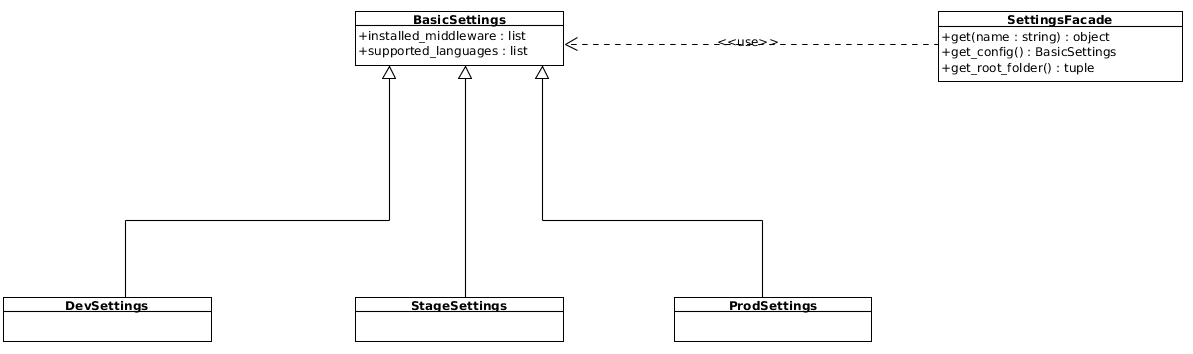
\includegraphics{settings.png}

As you can see, if you want to overwrite basic configuration you simply have to extend the class and set new values
for the attributes you want to overwrite.
\index{database\_config (fantastico.settings.BasicSettings attribute)}

\begin{fulllineitems}
\phantomsection\label{get_started/settings:fantastico.settings.BasicSettings.database_config}\pysigline{\bfcode{database\_config}}
This property holds the configuration of database. It is recommended to have all environment configured the same.
An exception can be done for host but the rest must remain the same. Below you can find an example of functional
configuration:

\begin{Verbatim}[commandchars=\\\{\}]
\PYG{n}{config} \PYG{o}{=} \PYG{p}{\PYGZob{}}\PYG{l+s}{\PYGZdq{}}\PYG{l+s}{drivername}\PYG{l+s}{\PYGZdq{}}\PYG{p}{:} \PYG{l+s}{\PYGZdq{}}\PYG{l+s}{mysql+mysqlconnector}\PYG{l+s}{\PYGZdq{}}\PYG{p}{,}
            \PYG{l+s}{\PYGZdq{}}\PYG{l+s}{username}\PYG{l+s}{\PYGZdq{}}\PYG{p}{:} \PYG{l+s}{\PYGZdq{}}\PYG{l+s}{fantastico}\PYG{l+s}{\PYGZdq{}}\PYG{p}{,}
            \PYG{l+s}{\PYGZdq{}}\PYG{l+s}{password}\PYG{l+s}{\PYGZdq{}}\PYG{p}{:} \PYG{l+s}{\PYGZdq{}}\PYG{l+s}{12345}\PYG{l+s}{\PYGZdq{}}\PYG{p}{,}
            \PYG{l+s}{\PYGZdq{}}\PYG{l+s}{port}\PYG{l+s}{\PYGZdq{}}\PYG{p}{:} \PYG{l+m+mi}{3306}\PYG{p}{,}
            \PYG{l+s}{\PYGZdq{}}\PYG{l+s}{host}\PYG{l+s}{\PYGZdq{}}\PYG{p}{:} \PYG{l+s}{\PYGZdq{}}\PYG{l+s}{localhost}\PYG{l+s}{\PYGZdq{}}\PYG{p}{,}
            \PYG{l+s}{\PYGZdq{}}\PYG{l+s}{database}\PYG{l+s}{\PYGZdq{}}\PYG{p}{:} \PYG{l+s}{\PYGZdq{}}\PYG{l+s}{fantastico}\PYG{l+s}{\PYGZdq{}}\PYG{p}{,}
            \PYG{l+s}{\PYGZdq{}}\PYG{l+s}{additional\PYGZus{}params}\PYG{l+s}{\PYGZdq{}}\PYG{p}{:} \PYG{p}{\PYGZob{}}\PYG{l+s}{\PYGZdq{}}\PYG{l+s}{charset}\PYG{l+s}{\PYGZdq{}}\PYG{p}{:} \PYG{l+s}{\PYGZdq{}}\PYG{l+s}{utf8}\PYG{l+s}{\PYGZdq{}}\PYG{p}{\PYGZcb{}}\PYG{p}{,}
            \PYG{l+s}{\PYGZdq{}}\PYG{l+s}{show\PYGZus{}sql}\PYG{l+s}{\PYGZdq{}}\PYG{p}{:} \PYG{n+nb+bp}{True}\PYG{p}{\PYGZcb{}}
\end{Verbatim}

As you can see, in your configuration you can influence many attributes used when configuring the driver / database.
\textbf{show\_sql} key tells orm engine from \textbf{Fantastico} to display all generated queries.

\end{fulllineitems}

\index{dev\_server\_host (fantastico.settings.BasicSettings attribute)}

\begin{fulllineitems}
\phantomsection\label{get_started/settings:fantastico.settings.BasicSettings.dev_server_host}\pysigline{\bfcode{dev\_server\_host}}
This property holds development server hostname. By default this is localhost.

\end{fulllineitems}

\index{dev\_server\_port (fantastico.settings.BasicSettings attribute)}

\begin{fulllineitems}
\phantomsection\label{get_started/settings:fantastico.settings.BasicSettings.dev_server_port}\pysigline{\bfcode{dev\_server\_port}}
This property holds development server port. By default this is 12000.

\end{fulllineitems}

\index{installed\_middleware (fantastico.settings.BasicSettings attribute)}

\begin{fulllineitems}
\phantomsection\label{get_started/settings:fantastico.settings.BasicSettings.installed_middleware}\pysigline{\bfcode{installed\_middleware}}
Property that holds all installed middlewares.

\end{fulllineitems}

\index{routes\_loaders (fantastico.settings.BasicSettings attribute)}

\begin{fulllineitems}
\phantomsection\label{get_started/settings:fantastico.settings.BasicSettings.routes_loaders}\pysigline{\bfcode{routes\_loaders}}
This property holds all routes loaders available.

\end{fulllineitems}

\index{supported\_languages (fantastico.settings.BasicSettings attribute)}

\begin{fulllineitems}
\phantomsection\label{get_started/settings:fantastico.settings.BasicSettings.supported_languages}\pysigline{\bfcode{supported\_languages}}
Property that holds all supported languages by this fantastico instance.

\end{fulllineitems}

\index{templates\_config (fantastico.settings.BasicSettings attribute)}

\begin{fulllineitems}
\phantomsection\label{get_started/settings:fantastico.settings.BasicSettings.templates_config}\pysigline{\bfcode{templates\_config}}
This property holds configuration of templates rendering engine. For the moment this influence how 
\href{http://jinja.pocoo.org/docs/}{Jinja2} acts.

\end{fulllineitems}


\end{fulllineitems}



\subsection{Create Dev configuration}
\label{get_started/settings:create-dev-configuration}
Let's imagine you want to create a custom dev configuration for your project. Below you can find the code for this:

\begin{Verbatim}[commandchars=\\\{\}]
\PYG{k}{class} \PYG{n+nc}{DevSettings}\PYG{p}{(}\PYG{n}{BasicSettings}\PYG{p}{)}\PYG{p}{:}
   \PYG{n+nd}{@property}
   \PYG{k}{def} \PYG{n+nf}{supported\PYGZus{}languages}\PYG{p}{(}\PYG{n+nb+bp}{self}\PYG{p}{)}\PYG{p}{:}
      \PYG{k}{return} \PYG{p}{[}\PYG{l+s}{\PYGZdq{}}\PYG{l+s}{en\PYGZus{}us}\PYG{l+s}{\PYGZdq{}}\PYG{p}{,} \PYG{l+s}{\PYGZdq{}}\PYG{l+s}{ro\PYGZus{}ro}\PYG{l+s}{\PYGZdq{}}\PYG{p}{]}
\end{Verbatim}

The above configuration actually overwrites supported languages. This mean that only en\_us is relevant for \textbf{Dev} environment.
You can do the same for \textbf{Stage}, \textbf{Prod} or any other custom configuration.


\subsection{Using a specifc configuration}
\label{get_started/settings:using-a-specifc-configuration}\index{SettingsFacade (class in fantastico.settings)}

\begin{fulllineitems}
\phantomsection\label{get_started/settings:fantastico.settings.SettingsFacade}\pysiglinewithargsret{\strong{class }\code{fantastico.settings.}\bfcode{SettingsFacade}}{\emph{environ=None}}{}
For using a specific fantastico configuration you need to do two simple steps:
\begin{itemize}
\item {} 
Set \textbf{FANTASTICO\_ACTIVE\_CONFIG} environment variable to the fully python qualified class name you want to use. E.g: {\hyperref[get_started/settings:fantastico.settings.BasicSettings]{\code{fantastico.settings.BasicSettings}}}

\item {} 
In your code, you can use the following snippet to access a specific setting:

\begin{Verbatim}[commandchars=\\\{\}]
\PYG{k+kn}{from} \PYG{n+nn}{fantastico.settings} \PYG{k+kn}{import} \PYG{n}{SettingsFacade}

\PYG{k}{print}\PYG{p}{(}\PYG{n}{SettingsFacade}\PYG{p}{(}\PYG{p}{)}\PYG{o}{.}\PYG{n}{get}\PYG{p}{(}\PYG{l+s}{\PYGZdq{}}\PYG{l+s}{installed\PYGZus{}middleware}\PYG{l+s}{\PYGZdq{}}\PYG{p}{)}\PYG{p}{)}
\end{Verbatim}

\end{itemize}

If no active configuration is set in the {\hyperref[get_started/settings:fantastico.settings.BasicSettings]{\code{fantastico.settings.BasicSettings}}} will be used.
\index{get() (fantastico.settings.SettingsFacade method)}

\begin{fulllineitems}
\phantomsection\label{get_started/settings:fantastico.settings.SettingsFacade.get}\pysiglinewithargsret{\bfcode{get}}{\emph{name}}{}
Method used to retrieve a setting value.
\begin{quote}\begin{description}
\item[{Parameters}] \leavevmode\begin{itemize}
\item {} 
\textbf{name} -- Setting name.

\item {} 
\textbf{type} -- string

\end{itemize}

\item[{Returns}] \leavevmode
The setting value.

\item[{Return type}] \leavevmode
object

\end{description}\end{quote}

\end{fulllineitems}

\index{get\_config() (fantastico.settings.SettingsFacade method)}

\begin{fulllineitems}
\phantomsection\label{get_started/settings:fantastico.settings.SettingsFacade.get_config}\pysiglinewithargsret{\bfcode{get\_config}}{}{}
Method used to return the active configuration which is used by this facade.
\begin{quote}\begin{description}
\item[{Return type}] \leavevmode
{\hyperref[get_started/settings:fantastico.settings.BasicSettings]{\code{fantastico.settings.BasicSettings}}}

\item[{Returns}] \leavevmode
Active configuration currently used.

\end{description}\end{quote}

\end{fulllineitems}

\index{get\_root\_folder() (fantastico.settings.SettingsFacade method)}

\begin{fulllineitems}
\phantomsection\label{get_started/settings:fantastico.settings.SettingsFacade.get_root_folder}\pysiglinewithargsret{\bfcode{get\_root\_folder}}{}{}
Method used to return the root folder of the current fantastico project (detected starting from settings)
profile used.

\end{fulllineitems}


\end{fulllineitems}



\section{Contribute}
\label{get_started/contribute:contribute}\label{get_started/contribute::doc}
Fantastico framework is open source so every contribution is welcome. For the moment we are looking for more developers willing to
contribute.


\subsection{Code contribution}
\label{get_started/contribute:code-contribution}
If you want to contribute with code to fantastico framework there are a simple set of rules that you must follow:
\begin{itemize}
\item {} 
Write unit tests (for the code / feature you are contributing).

\item {} 
Write integration tests (for the code / feature you are contributing).

\item {} 
Make sure your code is rated above 9.5 by pylint tool.

\item {} 
In addition integration tests and unit tests must cover 95\% of your code.

\end{itemize}

In order for each build to remain stable the following hard limits are imposed:
\begin{enumerate}
\item {} 
Unit tests must cover \textgreater{}= 95\% of the code.

\item {} 
Integration tests must cover \textgreater{}= 95\% of the code.

\item {} 
Code must be rated above 9.5 by pylint.

\item {} 
Everything must pass.

\end{enumerate}

When you push on master a set of jobs are cascaded executed:
\begin{enumerate}
\item {} 
Run all unit tests job.

\item {} 
Run all integration tests job (only if unit tests succeeds).

\item {} 
Generate documentation and publish it (only if integration tests job succeeds).

\end{enumerate}

You can follow the above build process by visiting
\href{http://jenkins.scrum-expert.ro:8080/job/fantastico-framework/}{Jenkins build}. Login with your github account and everything
should work smoothly.

In the end do not forget that in Fantastico framework we love to develop against a \textbf{stable} base. We really think code will have
high quality and zero bugs.


\subsubsection{Writing unit tests}
\label{get_started/contribute:writing-unit-tests}
For better understanding how to write unit tests see the documentation below:
\index{FantasticoUnitTestsCase (class in fantastico.tests.base\_case)}

\begin{fulllineitems}
\phantomsection\label{get_started/contribute:fantastico.tests.base_case.FantasticoUnitTestsCase}\pysiglinewithargsret{\strong{class }\code{fantastico.tests.base\_case.}\bfcode{FantasticoUnitTestsCase}}{\emph{methodName='runTest'}}{}
This is the base class that must be inherited by each unit test written for fantastico.

\begin{Verbatim}[commandchars=\\\{\}]
\PYG{k}{class} \PYG{n+nc}{SimpleUnitTest}\PYG{p}{(}\PYG{n}{FantasticoUnitTestsCase}\PYG{p}{)}\PYG{p}{:}
    \PYG{k}{def} \PYG{n+nf}{init}\PYG{p}{(}\PYG{n+nb+bp}{self}\PYG{p}{)}\PYG{p}{:}
        \PYG{n+nb+bp}{self}\PYG{o}{.}\PYG{n}{\PYGZus{}msg} \PYG{o}{=} \PYG{l+s}{\PYGZdq{}}\PYG{l+s}{Hello world}\PYG{l+s}{\PYGZdq{}}
        
    \PYG{k}{def} \PYG{n+nf}{test\PYGZus{}simple\PYGZus{}flow\PYGZus{}ok}\PYG{p}{(}\PYG{n+nb+bp}{self}\PYG{p}{)}\PYG{p}{:}
        \PYG{n+nb+bp}{self}\PYG{o}{.}\PYG{n}{assertEqual}\PYG{p}{(}\PYG{l+s}{\PYGZdq{}}\PYG{l+s}{Hello world}\PYG{l+s}{\PYGZdq{}}\PYG{p}{,} \PYG{n+nb+bp}{self}\PYG{o}{.}\PYG{n}{\PYGZus{}msg}\PYG{p}{)}
\end{Verbatim}
\index{\_get\_class\_root\_folder() (fantastico.tests.base\_case.FantasticoUnitTestsCase method)}

\begin{fulllineitems}
\phantomsection\label{get_started/contribute:fantastico.tests.base_case.FantasticoUnitTestsCase._get_class_root_folder}\pysiglinewithargsret{\bfcode{\_get\_class\_root\_folder}}{}{}
This methods determines the root folder under which the test is executed.

\end{fulllineitems}

\index{\_get\_root\_folder() (fantastico.tests.base\_case.FantasticoUnitTestsCase method)}

\begin{fulllineitems}
\phantomsection\label{get_started/contribute:fantastico.tests.base_case.FantasticoUnitTestsCase._get_root_folder}\pysiglinewithargsret{\bfcode{\_get\_root\_folder}}{}{}
This method determines the root folder under which core is executed.

\end{fulllineitems}

\index{setup\_once() (fantastico.tests.base\_case.FantasticoUnitTestsCase class method)}

\begin{fulllineitems}
\phantomsection\label{get_started/contribute:fantastico.tests.base_case.FantasticoUnitTestsCase.setup_once}\pysiglinewithargsret{\strong{classmethod }\bfcode{setup\_once}}{}{}
This method is overriden in order to correctly mock some dependencies:
\begin{itemize}
\item {} 
{\hyperref[features/mvc:fantastico.mvc.controller_decorators.Controller]{\code{fantastico.mvc.controller\_decorators.Controller}}}

\end{itemize}

\end{fulllineitems}


\end{fulllineitems}



\subsubsection{Writing integration tests}
\label{get_started/contribute:writing-integration-tests}
For better understanding how to write integration tests see the documentation below:
\index{FantasticoIntegrationTestCase (class in fantastico.tests.base\_case)}

\begin{fulllineitems}
\phantomsection\label{get_started/contribute:fantastico.tests.base_case.FantasticoIntegrationTestCase}\pysiglinewithargsret{\strong{class }\code{fantastico.tests.base\_case.}\bfcode{FantasticoIntegrationTestCase}}{\emph{methodName='runTest'}}{}
This is the base class that must be inherited by each integration test written for fantastico.

\begin{Verbatim}[commandchars=\\\{\}]
\PYG{k}{class} \PYG{n+nc}{SimpleIntegration}\PYG{p}{(}\PYG{n}{FantasticoIntegrationTestCase}\PYG{p}{)}\PYG{p}{:}
    \PYG{k}{def} \PYG{n+nf}{init}\PYG{p}{(}\PYG{n+nb+bp}{self}\PYG{p}{)}\PYG{p}{:}
        \PYG{n+nb+bp}{self}\PYG{o}{.}\PYG{n}{simple\PYGZus{}class} \PYG{o}{=} \PYG{p}{\PYGZob{}}\PYG{p}{\PYGZcb{}}
    
    \PYG{k}{def} \PYG{n+nf}{cleanup}\PYG{p}{(}\PYG{n+nb+bp}{self}\PYG{p}{)}\PYG{p}{:}
        \PYG{n+nb+bp}{self}\PYG{o}{.}\PYG{n}{simple\PYGZus{}class} \PYG{o}{=} \PYG{n+nb+bp}{None}
    
    \PYG{k}{def} \PYG{n+nf}{test\PYGZus{}simple\PYGZus{}ok}\PYG{p}{(}\PYG{n+nb+bp}{self}\PYG{p}{)}\PYG{p}{:}
        \PYG{k}{def} \PYG{n+nf}{do\PYGZus{}stuff}\PYG{p}{(}\PYG{n}{env}\PYG{p}{,} \PYG{n}{env\PYGZus{}cls}\PYG{p}{)}\PYG{p}{:}
            \PYG{n+nb+bp}{self}\PYG{o}{.}\PYG{n}{assertEqual}\PYG{p}{(}\PYG{n}{simple\PYGZus{}class}\PYG{p}{[}\PYG{n}{env}\PYG{p}{]}\PYG{p}{,} \PYG{n}{env\PYGZus{}cls}\PYG{p}{)}
            
        \PYG{n+nb+bp}{self}\PYG{o}{.}\PYG{n}{\PYGZus{}run\PYGZus{}test\PYGZus{}all\PYGZus{}envs}\PYG{p}{(}\PYG{n}{do\PYGZus{}stuff}\PYG{p}{)}
\end{Verbatim}

If you used this class you don't have to mind about restoring call methods from each middleware once they are wrapped
by fantastico app. This is a must because otherwise you will crash other tests.
\index{\_envs (fantastico.tests.base\_case.FantasticoIntegrationTestCase attribute)}

\begin{fulllineitems}
\phantomsection\label{get_started/contribute:fantastico.tests.base_case.FantasticoIntegrationTestCase._envs}\pysigline{\bfcode{\_envs}}
Private property that holds the environments against which we run the integration tests.

\end{fulllineitems}

\index{\_restore\_call\_methods() (fantastico.tests.base\_case.FantasticoIntegrationTestCase method)}

\begin{fulllineitems}
\phantomsection\label{get_started/contribute:fantastico.tests.base_case.FantasticoIntegrationTestCase._restore_call_methods}\pysiglinewithargsret{\bfcode{\_restore\_call\_methods}}{}{}
This method restore original call methods to all affected middlewares.

\end{fulllineitems}

\index{\_run\_test\_all\_envs() (fantastico.tests.base\_case.FantasticoIntegrationTestCase method)}

\begin{fulllineitems}
\phantomsection\label{get_started/contribute:fantastico.tests.base_case.FantasticoIntegrationTestCase._run_test_all_envs}\pysiglinewithargsret{\bfcode{\_run\_test\_all\_envs}}{\emph{callable\_obj}}{}
This method is used to execute a callable block of code on all environments. This is extremely useful for
avoid boiler plate code duplication and executing test logic against all environments.

\end{fulllineitems}

\index{\_save\_call\_methods() (fantastico.tests.base\_case.FantasticoIntegrationTestCase method)}

\begin{fulllineitems}
\phantomsection\label{get_started/contribute:fantastico.tests.base_case.FantasticoIntegrationTestCase._save_call_methods}\pysiglinewithargsret{\bfcode{\_save\_call\_methods}}{\emph{middlewares}}{}
This method save all call methods for each listed middleware so that later on they can be restored.

\end{fulllineitems}


\end{fulllineitems}

\index{DevServerIntegration (class in fantastico.server.tests.itest\_dev\_server)}

\begin{fulllineitems}
\phantomsection\label{get_started/contribute:fantastico.server.tests.itest_dev_server.DevServerIntegration}\pysiglinewithargsret{\strong{class }\code{fantastico.server.tests.itest\_dev\_server.}\bfcode{DevServerIntegration}}{\emph{methodName='runTest'}}{}
This class provides the foundation for writing integration tests that do http requests against a fantastico server.

\begin{Verbatim}[commandchars=\\\{\}]
\PYG{k}{class} \PYG{n+nc}{DummyLoaderIntegration}\PYG{p}{(}\PYG{n}{DevServerIntegration}\PYG{p}{)}\PYG{p}{:}
    \PYG{k}{def} \PYG{n+nf}{init}\PYG{p}{(}\PYG{n+nb+bp}{self}\PYG{p}{)}\PYG{p}{:}
        \PYG{n+nb+bp}{self}\PYG{o}{.}\PYG{n}{\PYGZus{}exception} \PYG{o}{=} \PYG{n+nb+bp}{None}

    \PYG{k}{def} \PYG{n+nf}{test\PYGZus{}server\PYGZus{}runs\PYGZus{}ok}\PYG{p}{(}\PYG{n+nb+bp}{self}\PYG{p}{)}\PYG{p}{:}
        \PYG{k}{def} \PYG{n+nf}{request\PYGZus{}logic}\PYG{p}{(}\PYG{n}{server}\PYG{p}{)}\PYG{p}{:}
            \PYG{n}{request} \PYG{o}{=} \PYG{n}{Request}\PYG{p}{(}\PYG{n+nb+bp}{self}\PYG{o}{.}\PYG{n}{\PYGZus{}get\PYGZus{}server\PYGZus{}base\PYGZus{}url}\PYG{p}{(}\PYG{n}{server}\PYG{p}{,} \PYG{n}{DummyRouteLoader}\PYG{o}{.}\PYG{n}{DUMMY\PYGZus{}ROUTE}\PYG{p}{)}\PYG{p}{)} 
            \PYG{k}{with} \PYG{n+nb+bp}{self}\PYG{o}{.}\PYG{n}{assertRaises}\PYG{p}{(}\PYG{n}{HTTPError}\PYG{p}{)} \PYG{k}{as} \PYG{n}{cm}\PYG{p}{:}
                \PYG{n}{urllib}\PYG{o}{.}\PYG{n}{request}\PYG{o}{.}\PYG{n}{urlopen}\PYG{p}{(}\PYG{n}{request}\PYG{p}{)}
                
            \PYG{n+nb+bp}{self}\PYG{o}{.}\PYG{n}{\PYGZus{}exception} \PYG{o}{=} \PYG{n}{cm}\PYG{o}{.}\PYG{n}{exception}
            
        \PYG{k}{def} \PYG{n+nf}{assert\PYGZus{}logic}\PYG{p}{(}\PYG{n}{server}\PYG{p}{)}\PYG{p}{:}
            \PYG{n+nb+bp}{self}\PYG{o}{.}\PYG{n}{assertEqual}\PYG{p}{(}\PYG{l+m+mi}{400}\PYG{p}{,} \PYG{n+nb+bp}{self}\PYG{o}{.}\PYG{n}{\PYGZus{}exception}\PYG{o}{.}\PYG{n}{code}\PYG{p}{)}
            \PYG{n+nb+bp}{self}\PYG{o}{.}\PYG{n}{assertEqual}\PYG{p}{(}\PYG{l+s}{\PYGZdq{}}\PYG{l+s}{Hello world.}\PYG{l+s}{\PYGZdq{}}\PYG{p}{,} \PYG{n+nb+bp}{self}\PYG{o}{.}\PYG{n}{\PYGZus{}exception}\PYG{o}{.}\PYG{n}{read}\PYG{p}{(}\PYG{p}{)}\PYG{o}{.}\PYG{n}{decode}\PYG{p}{(}\PYG{p}{)}\PYG{p}{)}                    
            
        \PYG{n+nb+bp}{self}\PYG{o}{.}\PYG{n}{\PYGZus{}run\PYGZus{}test\PYGZus{}all\PYGZus{}envs}\PYG{p}{(}\PYG{k}{lambda} \PYG{n}{env}\PYG{p}{,} \PYG{n}{settings\PYGZus{}cls}\PYG{p}{:} \PYG{n+nb+bp}{self}\PYG{o}{.}\PYG{n}{\PYGZus{}run\PYGZus{}test\PYGZus{}against\PYGZus{}dev\PYGZus{}server}\PYG{p}{(}\PYG{n}{request\PYGZus{}logic}\PYG{p}{,} \PYG{n}{assert\PYGZus{}logic}\PYG{p}{)}\PYG{p}{)}
        
        \PYG{c}{\PYGZsh{} you can also pass only request logic without assert logic}
        \PYG{c}{\PYGZsh{} self.\PYGZus{}run\PYGZus{}test\PYGZus{}all\PYGZus{}envs(lambda env, settings\PYGZus{}cls: self.\PYGZus{}run\PYGZus{}test\PYGZus{}against\PYGZus{}dev\PYGZus{}server(request\PYGZus{}logic))}
\end{Verbatim}

As you can see from above listed code, when you write a new integration test against Fantastico server you only need
to provide the request logic and assert logic functions. Request logic is executed while the server is up and running.
Assert logic is executed after the server has stopped.
\index{\_check\_server\_started() (fantastico.server.tests.itest\_dev\_server.DevServerIntegration method)}

\begin{fulllineitems}
\phantomsection\label{get_started/contribute:fantastico.server.tests.itest_dev_server.DevServerIntegration._check_server_started}\pysiglinewithargsret{\bfcode{\_check\_server\_started}}{\emph{server}}{}
This method holds the sanity checks to ensure a server is started correctly.

\end{fulllineitems}

\index{\_get\_server\_base\_url() (fantastico.server.tests.itest\_dev\_server.DevServerIntegration method)}

\begin{fulllineitems}
\phantomsection\label{get_started/contribute:fantastico.server.tests.itest_dev_server.DevServerIntegration._get_server_base_url}\pysiglinewithargsret{\bfcode{\_get\_server\_base\_url}}{\emph{server}, \emph{route}}{}
This method returns the absolute url for a given relative url (route).

\end{fulllineitems}

\index{\_run\_test\_against\_dev\_server() (fantastico.server.tests.itest\_dev\_server.DevServerIntegration method)}

\begin{fulllineitems}
\phantomsection\label{get_started/contribute:fantastico.server.tests.itest_dev_server.DevServerIntegration._run_test_against_dev_server}\pysiglinewithargsret{\bfcode{\_run\_test\_against\_dev\_server}}{\emph{request\_logic}, \emph{assert\_logic=None}}{}
This method provides a template for writing integration tests that requires a development server being active.
It accepts a request logic (code that actually do the http request) and an assert logic for making sure 
code is correct.

\end{fulllineitems}


\end{fulllineitems}



\section{Development mode}
\label{get_started/dev_mode::doc}\label{get_started/dev_mode:development-mode}
\textbf{Fantastico} framework is a web framework designed to be developers friendly. In order to simplify setup sequence, fantastico
provides a standalone WSGI compatible server that can be started from command line. This server is fully compliant with WSGI
standard. Below you can find some easy steps to achieve this:
\begin{enumerate}
\item {} 
Goto fantastico framework or project location

\item {} 
sh run\_dev\_server.sh

\end{enumerate}

This is it. Now you have a running fantastico server on which you can test your work.

By default, \textbf{Fantastico} dev server starts on port 12000, but you can customize it from
{\hyperref[get_started/settings:fantastico.settings.BasicSettings]{\code{fantastico.settings.BasicSettings}}}.


\subsection{Hot deploy}
\label{get_started/dev_mode:hot-deploy}
Currently, this is not implemented, but it is on todo list on short term.


\subsection{API}
\label{get_started/dev_mode:api}
For more information about Fantastico development server see the API below.
\index{DevServer (class in fantastico.server.dev\_server)}

\begin{fulllineitems}
\phantomsection\label{get_started/dev_mode:fantastico.server.dev_server.DevServer}\pysiglinewithargsret{\strong{class }\code{fantastico.server.dev\_server.}\bfcode{DevServer}}{\emph{settings\_facade=\textless{}class `fantastico.settings.SettingsFacade'\textgreater{}}}{}
This class provides a very simple wsgi http server that embeds Fantastico framework into it. As developer you can use
it to simply test your new components.
\index{start() (fantastico.server.dev\_server.DevServer method)}

\begin{fulllineitems}
\phantomsection\label{get_started/dev_mode:fantastico.server.dev_server.DevServer.start}\pysiglinewithargsret{\bfcode{start}}{\emph{build\_server=\textless{}function make\_server at 0x430dd10\textgreater{}}, \emph{app=\textless{}class `fantastico.middleware.fantastico\_app.FantasticoApp'\textgreater{}}}{}
This method starts a WSGI development server. All attributes like port, hostname and protocol are read from
configuration file.

\end{fulllineitems}

\index{started (fantastico.server.dev\_server.DevServer attribute)}

\begin{fulllineitems}
\phantomsection\label{get_started/dev_mode:fantastico.server.dev_server.DevServer.started}\pysigline{\bfcode{started}}
Property used to tell if development server is started or not.

\end{fulllineitems}

\index{stop() (fantastico.server.dev\_server.DevServer method)}

\begin{fulllineitems}
\phantomsection\label{get_started/dev_mode:fantastico.server.dev_server.DevServer.stop}\pysiglinewithargsret{\bfcode{stop}}{}{}
This method stops the current running server (if any available).

\end{fulllineitems}


\end{fulllineitems}



\subsection{Database config}
\label{get_started/dev_mode:database-config}
Usually you will use \textbf{Fantastico} framework together with a database. When we develop new core features of \textbf{Fantastico}
we use a sample database for integration. You can easily use it as well to play around:
\begin{enumerate}
\item {} 
Goto fantastico framework location

\item {} 
export MYSQL\_PASSWD=***** (your mysql password)

\item {} 
export MYSQL\_HOST=\textless{}hostname\textgreater{} (your mysql hostname: e.g localhost)

\item {} 
sh run\_setup\_db.sh

\end{enumerate}

\textbf{run\_setup\_db.sh} create an initial fantastico database and a user called fantastico identified by \textbf{12345} password. After
database is successfully created, it scans for all available \textbf{module\_setup.sql} files and execute them against newly created
database.


\chapter{Fantastico features}
\label{features/features::doc}\label{features/features:fantastico-features}

\section{Exceptions hierarchy}
\label{features/exceptions:exceptions-hierarchy}\label{features/exceptions::doc}\index{FantasticoError (class in fantastico.exceptions)}

\begin{fulllineitems}
\phantomsection\label{features/exceptions:fantastico.exceptions.FantasticoError}\pysigline{\strong{class }\code{fantastico.exceptions.}\bfcode{FantasticoError}}~
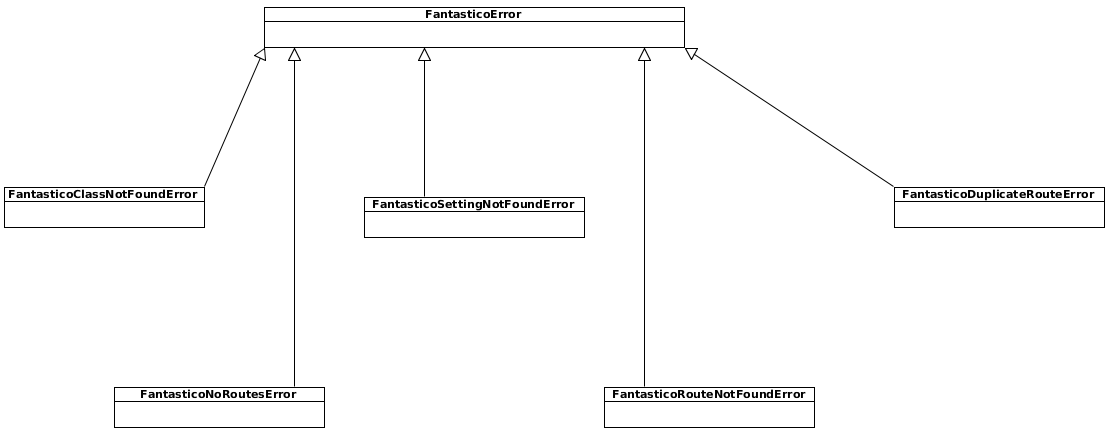
\includegraphics{exceptions.png}

\textbf{FantasticoError} is the base of all exceptions raised within fantastico framework. It describe common attributes that
each concrete fantastico exception must provide. By default all fantastico exceptions inherit FantasticoError exception. 
We do this because each raised unhandled FantasticoError is map to a specific exception response. This strategy guarantees
that at no moment errors will cause fantastico framework wsgi container to crash.

\end{fulllineitems}

\index{FantasticoControllerInvalidError (class in fantastico.exceptions)}

\begin{fulllineitems}
\phantomsection\label{features/exceptions:fantastico.exceptions.FantasticoControllerInvalidError}\pysigline{\strong{class }\code{fantastico.exceptions.}\bfcode{FantasticoControllerInvalidError}}
This exception is raised whenever a method is decorated with 
{\hyperref[features/mvc:fantastico.mvc.controller_decorators.Controller]{\code{fantastico.mvc.controller\_decorators.Controller}}} and the number of arguments is not correct. Usually
developer forgot to add request as argument to the controller.

\end{fulllineitems}

\index{FantasticoClassNotFoundError (class in fantastico.exceptions)}

\begin{fulllineitems}
\phantomsection\label{features/exceptions:fantastico.exceptions.FantasticoClassNotFoundError}\pysigline{\strong{class }\code{fantastico.exceptions.}\bfcode{FantasticoClassNotFoundError}}
This exception is raised whenever code tries to dynamically import and instantiate a class which can not be resolved.

\end{fulllineitems}

\index{FantasticoNotSupportedError (class in fantastico.exceptions)}

\begin{fulllineitems}
\phantomsection\label{features/exceptions:fantastico.exceptions.FantasticoNotSupportedError}\pysigline{\strong{class }\code{fantastico.exceptions.}\bfcode{FantasticoNotSupportedError}}
This exception is raised whenever code tries to do an operation that is  not supported.

\end{fulllineitems}

\index{FantasticoSettingNotFoundError (class in fantastico.exceptions)}

\begin{fulllineitems}
\phantomsection\label{features/exceptions:fantastico.exceptions.FantasticoSettingNotFoundError}\pysigline{\strong{class }\code{fantastico.exceptions.}\bfcode{FantasticoSettingNotFoundError}}
This exception is raised whenever code tries to obtain a setting that is not available in the current fantastico
configuration.

\end{fulllineitems}

\index{FantasticoDuplicateRouteError (class in fantastico.exceptions)}

\begin{fulllineitems}
\phantomsection\label{features/exceptions:fantastico.exceptions.FantasticoDuplicateRouteError}\pysigline{\strong{class }\code{fantastico.exceptions.}\bfcode{FantasticoDuplicateRouteError}}
This exception is usually raised by routing engine when it detects duplicate routes.

\end{fulllineitems}

\index{FantasticoNoRoutesError (class in fantastico.exceptions)}

\begin{fulllineitems}
\phantomsection\label{features/exceptions:fantastico.exceptions.FantasticoNoRoutesError}\pysigline{\strong{class }\code{fantastico.exceptions.}\bfcode{FantasticoNoRoutesError}}
This exception is usually raised by routing engine when no loaders are configured or no routes are registered.

\end{fulllineitems}

\index{FantasticoRouteNotFoundError (class in fantastico.exceptions)}

\begin{fulllineitems}
\phantomsection\label{features/exceptions:fantastico.exceptions.FantasticoRouteNotFoundError}\pysigline{\strong{class }\code{fantastico.exceptions.}\bfcode{FantasticoRouteNotFoundError}}
This exception is usually raised by routing engine when a requested url is not registered.

\end{fulllineitems}

\index{FantasticoNoRequestError (class in fantastico.exceptions)}

\begin{fulllineitems}
\phantomsection\label{features/exceptions:fantastico.exceptions.FantasticoNoRequestError}\pysigline{\strong{class }\code{fantastico.exceptions.}\bfcode{FantasticoNoRequestError}}
This exception is usually raised when some components try to use fantastico.request from WSGI environ before 
{\hyperref[features/request_response:fantastico.middleware.request_middleware.RequestMiddleware]{\code{fantastico.middleware.request\_middleware.RequestMiddleware}}} was executed.

\end{fulllineitems}

\index{FantasticoContentTypeError (class in fantastico.exceptions)}

\begin{fulllineitems}
\phantomsection\label{features/exceptions:fantastico.exceptions.FantasticoContentTypeError}\pysigline{\strong{class }\code{fantastico.exceptions.}\bfcode{FantasticoContentTypeError}}
This exception is usually thrown when a mismatch between request accept and response content type. In
Fantastico we think it's mandatory to fulfill requests correctly and to take in consideration sent headers.

\end{fulllineitems}

\index{FantasticoHttpVerbNotSupported (class in fantastico.exceptions)}

\begin{fulllineitems}
\phantomsection\label{features/exceptions:fantastico.exceptions.FantasticoHttpVerbNotSupported}\pysiglinewithargsret{\strong{class }\code{fantastico.exceptions.}\bfcode{FantasticoHttpVerbNotSupported}}{\emph{http\_verb}}{}
This exception is usually thrown when a route is accessed with an http verb which does not support.
\index{http\_verb (fantastico.exceptions.FantasticoHttpVerbNotSupported attribute)}

\begin{fulllineitems}
\phantomsection\label{features/exceptions:fantastico.exceptions.FantasticoHttpVerbNotSupported.http_verb}\pysigline{\bfcode{http\_verb}}
This property returns the http verb that caused the problems.

\end{fulllineitems}


\end{fulllineitems}

\index{FantasticoTemplateNotFoundError (class in fantastico.exceptions)}

\begin{fulllineitems}
\phantomsection\label{features/exceptions:fantastico.exceptions.FantasticoTemplateNotFoundError}\pysigline{\strong{class }\code{fantastico.exceptions.}\bfcode{FantasticoTemplateNotFoundError}}
This exception is usually thrown when a controller tries to load a template which it does not found.

\end{fulllineitems}

\index{FantasticoIncompatibleClassError (class in fantastico.exceptions)}

\begin{fulllineitems}
\phantomsection\label{features/exceptions:fantastico.exceptions.FantasticoIncompatibleClassError}\pysigline{\strong{class }\code{fantastico.exceptions.}\bfcode{FantasticoIncompatibleClassError}}
This exception is usually thrown when we want to decorate / inject / mixin a class into another class
that does not support it. For instance, we want to build a {\hyperref[features/mvc:fantastico.mvc.model_facade.ModelFacade]{\code{fantastico.mvc.model\_facade.ModelFacade}}}
with a class that does not extend \textbf{BASEMODEL.}

\end{fulllineitems}

\index{FantasticoDbError (class in fantastico.exceptions)}

\begin{fulllineitems}
\phantomsection\label{features/exceptions:fantastico.exceptions.FantasticoDbError}\pysigline{\strong{class }\code{fantastico.exceptions.}\bfcode{FantasticoDbError}}
This exception is usually thrown when a database exception occurs. For one good example where this is used see
{\hyperref[features/mvc:fantastico.mvc.model_facade.ModelFacade]{\code{fantastico.mvc.model\_facade.ModelFacade}}}.

\end{fulllineitems}

\index{FantasticoDbNotFoundError (class in fantastico.exceptions)}

\begin{fulllineitems}
\phantomsection\label{features/exceptions:fantastico.exceptions.FantasticoDbNotFoundError}\pysigline{\strong{class }\code{fantastico.exceptions.}\bfcode{FantasticoDbNotFoundError}}
This exception is usually thrown when an entity does not exist but we try to update it. For one good example where this is 
used see {\hyperref[features/mvc:fantastico.mvc.model_facade.ModelFacade]{\code{fantastico.mvc.model\_facade.ModelFacade}}}.

\end{fulllineitems}



\section{Request lifecycle}
\label{features/request_response:request-lifecycle}\label{features/request_response::doc}
In this document you can find how a request is processed by fantastico framework. By default WSGI applications use a dictionary
that contains various useful keys:
\begin{itemize}
\item {} 
HTTP Headers

\item {} 
HTTP Cookies

\item {} 
Helper keys (e.g file wrapper).

\end{itemize}

In fantastico we want to hide the complexity of this dictionary and allow developers to use some standardized objects. Fantastico
framework follows a Request / Response paradigm. This mean that for every single http request only one single http response will
be generated. Below, you can find a simple example of how requests are processed by fantastico framework:

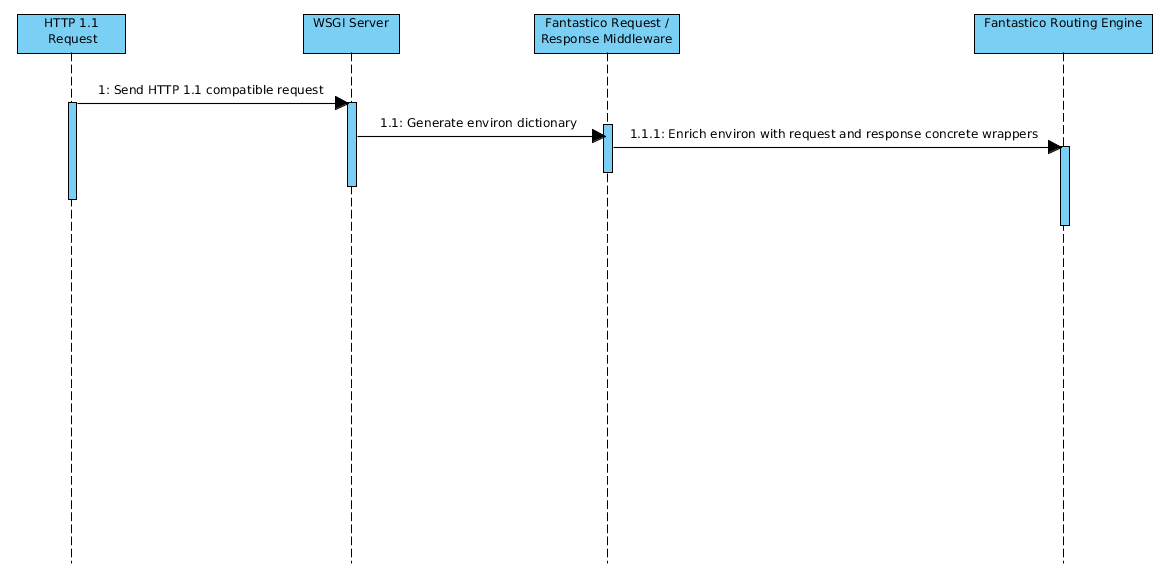
\includegraphics{request_response_sd.png}

In order to not reinvent the wheels fantastico relies on WebOb python framework in order to correctly generate request and
response objects. For more information read \href{http://docs.webob.org/en/latest/reference.html}{WebOB Doc}.


\subsection{Request middleware}
\label{features/request_response:request-middleware}
To have very good control of how WSGI environ is wrapped into \textbf{WebOb request} object a middleware component is configured. This
is the first middleware that is executed for every single http request.
\index{RequestMiddleware (class in fantastico.middleware.request\_middleware)}

\begin{fulllineitems}
\phantomsection\label{features/request_response:fantastico.middleware.request_middleware.RequestMiddleware}\pysiglinewithargsret{\strong{class }\code{fantastico.middleware.request\_middleware.}\bfcode{RequestMiddleware}}{\emph{app}}{}
This class provides the middleware responsible for converting wsgi environ dictionary into a request. The result is saved
into current WSGI environ under key \textbf{fantastico.request}.

\end{fulllineitems}



\subsection{Request context}
\label{features/request_response:request-context}
In comparison with WebOb \textbf{Fantastico} provides a nice improvement. For facilitating easy development of code, each fantastico
request has a special attribute called context. Below you can find the attributes of a request context object:
\begin{itemize}
\item {} 
settings facade ({\hyperref[get_started/settings::doc]{\emph{Fantastico settings}}})

\item {} 
session (not yet supported)

\item {} 
\textbf{language} The current preferred by user. This is determined based on user lang header.

\item {} 
user (not yet supported)

\end{itemize}
\index{RequestContext (class in fantastico.middleware.request\_context)}

\begin{fulllineitems}
\phantomsection\label{features/request_response:fantastico.middleware.request_context.RequestContext}\pysiglinewithargsret{\strong{class }\code{fantastico.middleware.request\_context.}\bfcode{RequestContext}}{\emph{settings}, \emph{language}}{}
This class holds various attributes useful giving a context to an http request. Among other things we need 
to be able to access current language, current session and possible current user profile.
\index{language (fantastico.middleware.request\_context.RequestContext attribute)}

\begin{fulllineitems}
\phantomsection\label{features/request_response:fantastico.middleware.request_context.RequestContext.language}\pysigline{\bfcode{language}}
Property that holds the current language that must be used during this request.

\end{fulllineitems}

\index{settings (fantastico.middleware.request\_context.RequestContext attribute)}

\begin{fulllineitems}
\phantomsection\label{features/request_response:fantastico.middleware.request_context.RequestContext.settings}\pysigline{\bfcode{settings}}
Property that holds the current settings facade used for accessing fantastico configuration.

\end{fulllineitems}


\end{fulllineitems}



\subsection{Obtain request language}
\label{features/request_response:obtain-request-language}\index{Language (class in fantastico.locale.language)}

\begin{fulllineitems}
\phantomsection\label{features/request_response:fantastico.locale.language.Language}\pysiglinewithargsret{\strong{class }\code{fantastico.locale.language.}\bfcode{Language}}{\emph{code}}{}
Class used to define how does language object looks like. There are various use cases for using language but
the simplest one is in request context object:

\begin{Verbatim}[commandchars=\\\{\}]
\PYG{n}{language} \PYG{o}{=} \PYG{n}{request}\PYG{o}{.}\PYG{n}{context}\PYG{o}{.}\PYG{n}{language}

\PYG{k}{if} \PYG{n}{language}\PYG{o}{.}\PYG{n}{code} \PYG{o}{=} \PYG{l+s}{\PYGZdq{}}\PYG{l+s}{en\PYGZus{}us}\PYG{l+s}{\PYGZdq{}}\PYG{p}{:}
   \PYG{k}{print}\PYG{p}{(}\PYG{l+s}{\PYGZdq{}}\PYG{l+s}{English (US) language}\PYG{l+s}{\PYGZdq{}}\PYG{p}{)}\PYG{o}{.}
\PYG{k}{else}\PYG{p}{:}
   \PYG{k}{raise} \PYG{n+ne}{Exception}\PYG{p}{(}\PYG{l+s}{\PYGZdq{}}\PYG{l+s}{Language }\PYG{l+s+si}{\PYGZpc{}s}\PYG{l+s}{ is not supported.}\PYG{l+s}{\PYGZdq{}} \PYG{o}{\PYGZpc{}} \PYG{n}{language}\PYG{o}{.}\PYG{n}{code}\PYG{p}{)}
\end{Verbatim}
\index{code (fantastico.locale.language.Language attribute)}

\begin{fulllineitems}
\phantomsection\label{features/request_response:fantastico.locale.language.Language.code}\pysigline{\bfcode{code}}
Property that holds the language code. This is readonly because once instantiated we mustn't be able to change it.

\end{fulllineitems}


\end{fulllineitems}



\subsection{Obtain settings using request}
\label{features/request_response:obtain-settings-using-request}
It is recommended to use \emph{request.context} object to obtain fantastico settings. This hides the complexity of choosing the right
configuration and accessing attributes from it.

\begin{Verbatim}[commandchars=\\\{\}]
\PYG{n}{installed\PYGZus{}middleware} \PYG{o}{=} \PYG{n}{request}\PYG{o}{.}\PYG{n}{context}\PYG{o}{.}\PYG{n}{settings}\PYG{o}{.}\PYG{n}{get}\PYG{p}{(}\PYG{l+s}{\PYGZdq{}}\PYG{l+s}{installed\PYGZus{}middleware}\PYG{l+s}{\PYGZdq{}}\PYG{p}{)}

\PYG{k}{print}\PYG{p}{(}\PYG{n}{installed\PYGZus{}middleware}\PYG{p}{)}
\end{Verbatim}

For more information about how to configure \textbf{Fantastico} please read {\hyperref[get_started/settings::doc]{\emph{Fantastico settings}}}.


\section{Routing engine}
\label{features/routing_engine:routing-engine}\label{features/routing_engine::doc}
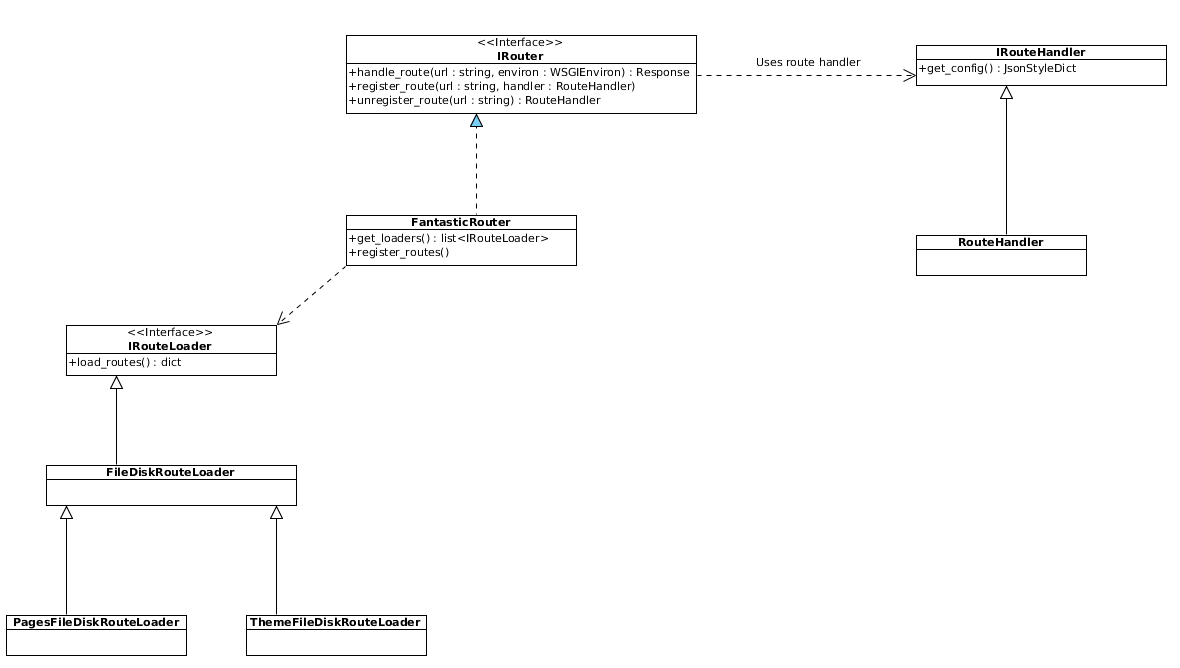
\includegraphics{routing_engine.png}

Fantastico routing engine is design by having extensibility in mind. Below you can find the list of concerns for routing engine:
\begin{enumerate}
\item {} 
Support multiple sources for routes.

\item {} 
Load all available routes.

\item {} 
Select the controller that can handle the request route (if any available).

\end{enumerate}
\index{Router (class in fantastico.routing\_engine.router)}

\begin{fulllineitems}
\phantomsection\label{features/routing_engine:fantastico.routing_engine.router.Router}\pysiglinewithargsret{\strong{class }\code{fantastico.routing\_engine.router.}\bfcode{Router}}{\emph{settings\_facade=\textless{}class `fantastico.settings.SettingsFacade'\textgreater{}}}{}
This class is used for registering all available routes by using all registered loaders.
\index{get\_loaders() (fantastico.routing\_engine.router.Router method)}

\begin{fulllineitems}
\phantomsection\label{features/routing_engine:fantastico.routing_engine.router.Router.get_loaders}\pysiglinewithargsret{\bfcode{get\_loaders}}{}{}
Method used to retrieve all available loaders. If loaders are not currently instantiated they are by these method.
This method also supports multi threaded workers mode of wsgi with really small memory footprint. It uses an internal
lock so that it makes sure available loaders are instantiated only once per wsgi worker.

\end{fulllineitems}

\index{handle\_route() (fantastico.routing\_engine.router.Router method)}

\begin{fulllineitems}
\phantomsection\label{features/routing_engine:fantastico.routing_engine.router.Router.handle_route}\pysiglinewithargsret{\bfcode{handle\_route}}{\emph{url}, \emph{environ}}{}
Method used to identify the given url method handler. It enrich the environ dictionary with a new entry that
holds a controller instance and a function to be executed from that controller.

\end{fulllineitems}

\index{register\_routes() (fantastico.routing\_engine.router.Router method)}

\begin{fulllineitems}
\phantomsection\label{features/routing_engine:fantastico.routing_engine.router.Router.register_routes}\pysiglinewithargsret{\bfcode{register\_routes}}{}{}
Method used to register all routes from all loaders. If the loaders are not yet initialized this method will first
load all available loaders and then it will register all available routes. Also, this method initialize available routes
only once when it is first invoked.

\end{fulllineitems}


\end{fulllineitems}



\subsection{Routes loaders}
\label{features/routing_engine:routes-loaders}
Fantastico routing engine is designed so that routes can be loaded from multiple sources (database, disk locations, and others).
This give huge extensibility so that developers can use Fantastico in various scenarios:
\begin{itemize}
\item {} 
Create a CMS that allows people to create new pages (mapping between page url / controller) is hold in database. Just by
adding a simple loader in which the business logic is encapsulated allows routing engine extension.

\item {} 
Create a blog that loads articles from disk.

\end{itemize}

I am sure you can find other use cases in which you benefit from this extension point.


\subsection{How to write a new route loader}
\label{features/routing_engine:how-to-write-a-new-route-loader}
Before digging in further details see the RouteLoader class documentation below:
\index{RouteLoader (class in fantastico.routing\_engine.routing\_loaders)}

\begin{fulllineitems}
\phantomsection\label{features/routing_engine:fantastico.routing_engine.routing_loaders.RouteLoader}\pysiglinewithargsret{\strong{class }\code{fantastico.routing\_engine.routing\_loaders.}\bfcode{RouteLoader}}{\emph{settings\_facade}}{}
This class provides the contract that must be provided by each concrete implementation. Each route loader is responsible
for implementing its own business logic for loading routes.

\begin{Verbatim}[commandchars=\\\{\}]
\PYG{k}{class} \PYG{n+nc}{DummyRouteLoader}\PYG{p}{(}\PYG{n}{RouteLoader}\PYG{p}{)}\PYG{p}{:}
    \PYG{k}{def} \PYG{n+nf}{\PYGZus{}\PYGZus{}init\PYGZus{}\PYGZus{}}\PYG{p}{(}\PYG{n+nb+bp}{self}\PYG{p}{,} \PYG{n}{settings\PYGZus{}facade}\PYG{p}{)}\PYG{p}{:}
        \PYG{n}{self\PYGZus{}settings\PYGZus{}facade} \PYG{o}{=} \PYG{n}{settings\PYGZus{}facade}
        
    \PYG{k}{def} \PYG{n+nf}{load\PYGZus{}routes}\PYG{p}{(}\PYG{n+nb+bp}{self}\PYG{p}{)}\PYG{p}{:}
        \PYG{k}{return} \PYG{p}{\PYGZob{}}\PYG{l+s}{\PYGZdq{}}\PYG{l+s}{/index.html}\PYG{l+s}{\PYGZdq{}}\PYG{p}{:} \PYG{p}{\PYGZob{}}\PYG{l+s}{\PYGZdq{}}\PYG{l+s}{method}\PYG{l+s}{\PYGZdq{}}\PYG{p}{:} \PYG{l+s}{\PYGZdq{}}\PYG{l+s}{fantastico.plugins.static\PYGZus{}assets.StaticAssetsController.resolve\PYGZus{}text}\PYG{l+s}{\PYGZdq{}}\PYG{p}{,}
                                \PYG{l+s}{\PYGZdq{}}\PYG{l+s}{http\PYGZus{}verbs}\PYG{l+s}{\PYGZdq{}}\PYG{p}{:} \PYG{p}{[}\PYG{l+s}{\PYGZdq{}}\PYG{l+s}{GET}\PYG{l+s}{\PYGZdq{}}\PYG{p}{]}\PYG{p}{\PYGZcb{}}\PYG{p}{,}
                \PYG{l+s}{\PYGZdq{}}\PYG{l+s}{/images/image.png}\PYG{l+s}{\PYGZdq{}}\PYG{p}{:} \PYG{p}{\PYGZob{}}\PYG{l+s}{\PYGZdq{}}\PYG{l+s}{method}\PYG{l+s}{\PYGZdq{}}\PYG{p}{:} \PYG{l+s}{\PYGZdq{}}\PYG{l+s}{fantastico.plugins.static\PYGZus{}assets.StaticAssetsController.resolve\PYGZus{}binary}\PYG{l+s}{\PYGZdq{}}\PYG{p}{,}
                                      \PYG{l+s}{\PYGZdq{}}\PYG{l+s}{http\PYGZus{}verbs}\PYG{l+s}{\PYGZdq{}}\PYG{p}{:} \PYG{p}{[}\PYG{l+s}{\PYGZdq{}}\PYG{l+s}{GET}\PYG{l+s}{\PYGZdq{}}\PYG{p}{]}\PYG{p}{\PYGZcb{}}
\end{Verbatim}
\index{load\_routes() (fantastico.routing\_engine.routing\_loaders.RouteLoader method)}

\begin{fulllineitems}
\phantomsection\label{features/routing_engine:fantastico.routing_engine.routing_loaders.RouteLoader.load_routes}\pysiglinewithargsret{\bfcode{load\_routes}}{}{}
This method must be overriden by each concrete implementation so that all loaded routes can be handled by
fantastico routing engine middleware.

\end{fulllineitems}


\end{fulllineitems}


As you can, each concrete route loader receives in the constructor settings facade that can be used to access fantastico settings.
In the code example above, DummyRouteLoader maps a list of urls to a controller method that can be used to render it. Keep in
mind that a route loader is a stateless component and it can't in anyway determine the wsgi environment in which it is used. In
addition this design decision also make sure clear separation of concerned is followed.

Once your \textbf{RouteLoader} implementation is ready you must register it into settings profile. The safest bet is to add it into
BaseSettings provider. For more information read {\hyperref[get_started/settings::doc]{\emph{Fantastico settings}}}.


\subsection{Configuring available loaders}
\label{features/routing_engine:configuring-available-loaders}
You can find all available loaders for the framework configured in your settings profile. You can find below a sample
configuration of available loaders:

\begin{Verbatim}[commandchars=\\\{\}]
\PYG{k}{class} \PYG{n+nc}{CustomSettings}\PYG{p}{(}\PYG{n}{BasicSettings}\PYG{p}{)}\PYG{p}{:}
    \PYG{n+nd}{@property}
    \PYG{k}{def} \PYG{n+nf}{routes\PYGZus{}loaders}\PYG{p}{(}\PYG{n+nb+bp}{self}\PYG{p}{)}\PYG{p}{:}
        \PYG{k}{return} \PYG{p}{[}\PYG{l+s}{\PYGZdq{}}\PYG{l+s}{fantastico.routing\PYGZus{}engine.custom\PYGZus{}loader.CustomLoader}\PYG{l+s}{\PYGZdq{}}\PYG{p}{]}
\end{Verbatim}

The above configuration tells \textbf{Fantastico routing engine} that only CustomLoader is a source of routes. If you want to learn
more about multiple configurations please read {\hyperref[get_started/settings::doc]{\emph{Fantastico settings}}}.


\subsection{DummyRouteLoader}
\label{features/routing_engine:dummyrouteloader}\index{DummyRouteLoader (class in fantastico.routing\_engine.dummy\_routeloader)}

\begin{fulllineitems}
\phantomsection\label{features/routing_engine:fantastico.routing_engine.dummy_routeloader.DummyRouteLoader}\pysiglinewithargsret{\strong{class }\code{fantastico.routing\_engine.dummy\_routeloader.}\bfcode{DummyRouteLoader}}{\emph{settings\_facade}}{}
This class represents an example of how to write a route loader. \textbf{DummyRouteLoader} is available in all configurations
and it provides a single route to the routing engine: \emph{/dummy/route/loader/test}. Integration tests rely on this loader
to be configured in each available profile.
\index{display\_test() (fantastico.routing\_engine.dummy\_routeloader.DummyRouteLoader method)}

\begin{fulllineitems}
\phantomsection\label{features/routing_engine:fantastico.routing_engine.dummy_routeloader.DummyRouteLoader.display_test}\pysiglinewithargsret{\bfcode{display\_test}}{\emph{request}}{}
This method handles \textbf{/dummy/route/loader/test route}. It is expected to receive a response with status code 400.
We do this for being able to test rendering and also avoid false positive security scans messages.

\end{fulllineitems}


\end{fulllineitems}



\subsection{Routing middleware}
\label{features/routing_engine:routing-middleware}
\textbf{Fantastico} routing engine is designed as a standalone component. In order to be able to integrate it into Fantastico request
lifecycle (:doc:/features/request\_response.) we need an adapter component.
\index{RoutingMiddleware (class in fantastico.middleware.routing\_middleware)}

\begin{fulllineitems}
\phantomsection\label{features/routing_engine:fantastico.middleware.routing_middleware.RoutingMiddleware}\pysiglinewithargsret{\strong{class }\code{fantastico.middleware.routing\_middleware.}\bfcode{RoutingMiddleware}}{\emph{app}, \emph{router\_cls=\textless{}class `fantastico.routing\_engine.router.Router'\textgreater{}}}{}
Class used to integrate routing engine fantastico component into request / response lifecycle. This middleware is 
responsible for:
\begin{enumerate}
\item {} 
instantiating the router component and make it available to other components / middlewares through WSGI environment.

\item {} 
register all configured fantastico loaders ({\hyperref[features/routing_engine:fantastico.routing_engine.router.Router.get_loaders]{\code{fantastico.routing\_engine.router.Router.get\_loaders()}}}).

\item {} 
register all available routes ({\hyperref[features/routing_engine:fantastico.routing_engine.router.Router.register_routes]{\code{fantastico.routing\_engine.router.Router.register\_routes()}}}).

\item {} 
handle route requests ({\hyperref[features/routing_engine:fantastico.routing_engine.router.Router.handle_route]{\code{fantastico.routing\_engine.router.Router.handle\_route()}}}).

\end{enumerate}

It is important to understand that routing middleware assume a \textbf{WebOb request} available into WSGI environ. Otherwise, 
{\hyperref[features/exceptions:fantastico.exceptions.FantasticoNoRequestError]{\code{fantastico.exceptions.FantasticoNoRequestError}}} will be thrown. You can read more about request middleware 
at {\hyperref[features/request_response::doc]{\emph{Request lifecycle}}}.

\end{fulllineitems}



\section{Model View Controller}
\label{features/mvc:model-view-controller}\label{features/mvc::doc}
\textbf{Fantastico} framework provides quite a powerful model - view - controller implementation. Here you can find details about
design decisions and how to benefit from it.


\subsection{Classic approach}
\label{features/mvc:classic-approach}
Usually when you want to work with models as understood by MVC pattern you have in many cases boiler plate code:
\begin{enumerate}
\item {} 
Write your model class (or entity)

\item {} 
Write a repository that provides various methods for this model class.

\item {} 
Write a facade that works with the repository.

\item {} 
Write a web service / page that relies on the facade.

\item {} 
Write one or multiple views.

\end{enumerate}

As this is usually a good in theory, in practice you will see that many methods from facade are converting a data transfer object
to an entity and pass it down to repository.


\subsection{Fantastico approach}
\label{features/mvc:fantastico-approach}
\textbf{Fantastico} framework provides an alternative to this classic approach (you can still work in the old way if you really really
want).
\index{Controller (class in fantastico.mvc.controller\_decorators)}

\begin{fulllineitems}
\phantomsection\label{features/mvc:fantastico.mvc.controller_decorators.Controller}\pysiglinewithargsret{\strong{class }\code{fantastico.mvc.controller\_decorators.}\bfcode{Controller}}{\emph{url}, \emph{method='GET'}, \emph{models=None}, \emph{model\_facade=\textless{}class `fantastico.mvc.model\_facade.ModelFacade'\textgreater{}}}{}
This class provides a decorator for magically registering methods as route handlers. This is an extremely important
piece of Fantastico framework because it simplifies the way you as developer can define mapping between a method that
must be executed when an http request to an url is made:

\begin{Verbatim}[commandchars=\\\{\}]
\PYG{n+nd}{@ControllerProvider}\PYG{p}{(}\PYG{p}{)}
\PYG{k}{class} \PYG{n+nc}{BlogsController}\PYG{p}{(}\PYG{n}{BaseController}\PYG{p}{)}\PYG{p}{:}        
    \PYG{n+nd}{@Controller}\PYG{p}{(}\PYG{n}{url}\PYG{o}{=}\PYG{l+s}{\PYGZdq{}}\PYG{l+s}{/blogs/}\PYG{l+s}{\PYGZdq{}}\PYG{p}{,} \PYG{n}{method}\PYG{o}{=}\PYG{l+s}{\PYGZdq{}}\PYG{l+s}{GET}\PYG{l+s}{\PYGZdq{}}\PYG{p}{,} 
                \PYG{n}{models}\PYG{o}{=}\PYG{p}{\PYGZob{}}\PYG{l+s}{\PYGZdq{}}\PYG{l+s}{Blog}\PYG{l+s}{\PYGZdq{}}\PYG{p}{:} \PYG{l+s}{\PYGZdq{}}\PYG{l+s}{fantastico.plugins.blog.models.blog.Blog}\PYG{l+s}{\PYGZdq{}}\PYG{p}{]}\PYG{p}{)}
    \PYG{k}{def} \PYG{n+nf}{list\PYGZus{}blogs}\PYG{p}{(}\PYG{n+nb+bp}{self}\PYG{p}{,} \PYG{n}{request}\PYG{p}{)}\PYG{p}{:}
        \PYG{n}{Blog} \PYG{o}{=} \PYG{n}{request}\PYG{o}{.}\PYG{n}{models}\PYG{o}{.}\PYG{n}{Blog}
    
        \PYG{n}{blogs} \PYG{o}{=} \PYG{n}{Blog}\PYG{o}{.}\PYG{n}{get\PYGZus{}records\PYGZus{}paged}\PYG{p}{(}\PYG{n}{start\PYGZus{}record}\PYG{o}{=}\PYG{l+m+mi}{0}\PYG{p}{,} \PYG{n}{end\PYGZus{}record}\PYG{o}{=}\PYG{l+m+mi}{5}\PYG{p}{,} 
                               \PYG{n}{sort\PYGZus{}expr}\PYG{o}{=}\PYG{p}{[}\PYG{n}{ModelSort}\PYG{p}{(}\PYG{n}{Blog}\PYG{o}{.}\PYG{n}{model\PYGZus{}cls}\PYG{o}{.}\PYG{n}{create\PYGZus{}date}\PYG{p}{,} \PYG{n}{ModelSort}\PYG{o}{.}\PYG{n}{ASC}\PYG{p}{,}
                                          \PYG{n}{ModelSort}\PYG{p}{(}\PYG{n}{Blog}\PYG{o}{.}\PYG{n}{model\PYGZus{}cls}\PYG{o}{.}\PYG{n}{title}\PYG{p}{,} \PYG{n}{ModelSort}\PYG{o}{.}\PYG{n}{DESC}\PYG{p}{)}\PYG{p}{]}\PYG{p}{,}
                               \PYG{n}{filter\PYGZus{}expr}\PYG{o}{=}\PYG{n}{ModelFilterAnd}\PYG{p}{(}
                                               \PYG{n}{ModelFilter}\PYG{p}{(}\PYG{n}{Blog}\PYG{o}{.}\PYG{n}{model\PYGZus{}cls}\PYG{o}{.}\PYG{n}{id}\PYG{p}{,} \PYG{l+m+mi}{1}\PYG{p}{,} \PYG{n}{ModelFilter}\PYG{o}{.}\PYG{n}{GT}\PYG{p}{)}\PYG{p}{,}
                                               \PYG{n}{ModelFilter}\PYG{p}{(}\PYG{n}{Blog}\PYG{o}{.}\PYG{n}{model\PYGZus{}cls}\PYG{o}{.}\PYG{n}{id}\PYG{p}{,} \PYG{l+m+mi}{5}\PYG{p}{,} \PYG{n}{ModelFilter}\PYG{o}{.}\PYG{n}{LT}\PYG{p}{)}\PYG{p}{)}\PYG{p}{)}\PYG{p}{)}
    
        \PYG{k}{return} \PYG{n}{Response}\PYG{p}{(}\PYG{n}{blogs}\PYG{p}{)}
\end{Verbatim}

The above code assume the following:
\begin{enumerate}
\item {} 
As developer you created a model called blog (this is already mapped to some sort of storage).

\item {} 
Fantastico framework generate the facade automatically (and you never have to know anything about underlining repository).

\item {} 
Fantastico framework takes care of data conversion.

\item {} 
As developer you create the method that knows how to handle \textbf{/blog/} url.

\item {} 
Write your view.

\end{enumerate}

Below you can find the design for MVC provided by \textbf{Fantastico} framework:

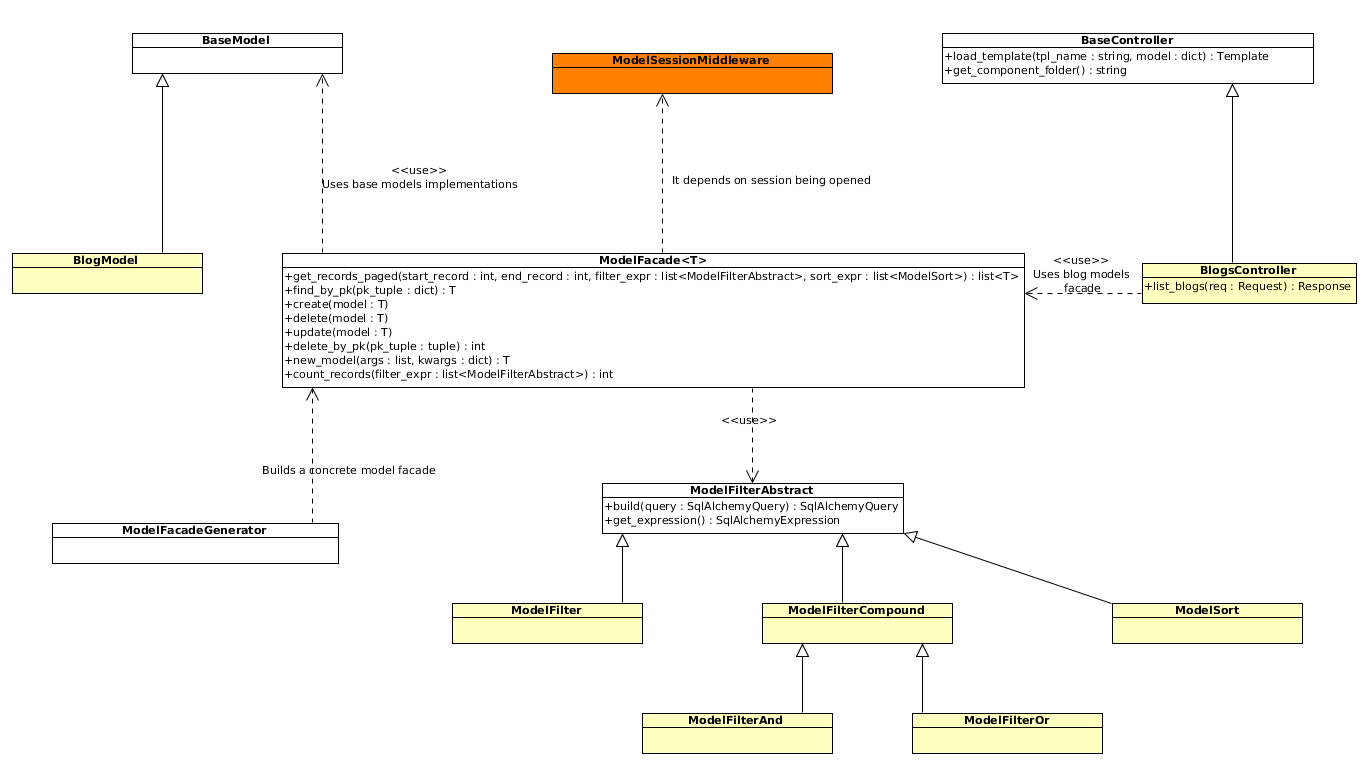
\includegraphics{mvc.png}
\index{fn\_handler (fantastico.mvc.controller\_decorators.Controller attribute)}

\begin{fulllineitems}
\phantomsection\label{features/mvc:fantastico.mvc.controller_decorators.Controller.fn_handler}\pysigline{\bfcode{fn\_handler}}
This property retrieves the method which is executed by this controller.

\end{fulllineitems}

\index{get\_registered\_routes() (fantastico.mvc.controller\_decorators.Controller class method)}

\begin{fulllineitems}
\phantomsection\label{features/mvc:fantastico.mvc.controller_decorators.Controller.get_registered_routes}\pysiglinewithargsret{\strong{classmethod }\bfcode{get\_registered\_routes}}{}{}
This class methods retrieve all registered routes through Controller decorator.

\end{fulllineitems}

\index{method (fantastico.mvc.controller\_decorators.Controller attribute)}

\begin{fulllineitems}
\phantomsection\label{features/mvc:fantastico.mvc.controller_decorators.Controller.method}\pysigline{\bfcode{method}}
This property retrieves the method(s) for which this controller can be invoked. Most of the time only one value is
retrieved.

\end{fulllineitems}

\index{models (fantastico.mvc.controller\_decorators.Controller attribute)}

\begin{fulllineitems}
\phantomsection\label{features/mvc:fantastico.mvc.controller_decorators.Controller.models}\pysigline{\bfcode{models}}
This property retrieves all the models required by this controller in order to work correctly.

\end{fulllineitems}

\index{url (fantastico.mvc.controller\_decorators.Controller attribute)}

\begin{fulllineitems}
\phantomsection\label{features/mvc:fantastico.mvc.controller_decorators.Controller.url}\pysigline{\bfcode{url}}
This property retrieves the url used when registering this controller.

\end{fulllineitems}


\end{fulllineitems}


If you want to find more details and use cases for controller read {\hyperref[features/mvc:core-controller-section]{\emph{Controller}}} section.


\subsection{Model}
\label{features/mvc:model}
A model is a very simple object that inherits \code{fantastico.mvc.models.BaseModel}.

In order for models to work correctly and to be injected correctly into controller you must make sure you have
a valid database configuration in your settings file. By default, {\hyperref[get_started/settings:fantastico.settings.BasicSettings]{\code{fantastico.settings.BasicSettings}}} provides a usable
database configuration.

\begin{Verbatim}[commandchars=\\\{\}]
\PYG{c}{\PYGZsh{} fantastico.settings.BasicSettings}
\PYG{n+nd}{@property}
\PYG{k}{def} \PYG{n+nf}{database\PYGZus{}config}\PYG{p}{(}\PYG{n+nb+bp}{self}\PYG{p}{)}\PYG{p}{:}
    \PYG{k}{return} \PYG{p}{\PYGZob{}}\PYG{l+s}{\PYGZdq{}}\PYG{l+s}{drivername}\PYG{l+s}{\PYGZdq{}}\PYG{p}{:} \PYG{l+s}{\PYGZdq{}}\PYG{l+s}{mysql+mysqldb}\PYG{l+s}{\PYGZdq{}}\PYG{p}{,}
            \PYG{l+s}{\PYGZdq{}}\PYG{l+s}{username}\PYG{l+s}{\PYGZdq{}}\PYG{p}{:} \PYG{l+s}{\PYGZdq{}}\PYG{l+s}{fantastico}\PYG{l+s}{\PYGZdq{}}\PYG{p}{,}
            \PYG{l+s}{\PYGZdq{}}\PYG{l+s}{password}\PYG{l+s}{\PYGZdq{}}\PYG{p}{:} \PYG{l+s}{\PYGZdq{}}\PYG{l+s}{12345}\PYG{l+s}{\PYGZdq{}}\PYG{p}{,}
            \PYG{l+s}{\PYGZdq{}}\PYG{l+s}{host}\PYG{l+s}{\PYGZdq{}}\PYG{p}{:} \PYG{l+s}{\PYGZdq{}}\PYG{l+s}{localhost}\PYG{l+s}{\PYGZdq{}}\PYG{p}{,}
            \PYG{l+s}{\PYGZdq{}}\PYG{l+s}{port}\PYG{l+s}{\PYGZdq{}}\PYG{p}{:} \PYG{l+m+mi}{3306}\PYG{p}{,}
            \PYG{l+s}{\PYGZdq{}}\PYG{l+s}{database}\PYG{l+s}{\PYGZdq{}}\PYG{p}{:} \PYG{l+s}{\PYGZdq{}}\PYG{l+s}{fantastico}\PYG{l+s}{\PYGZdq{}}\PYG{p}{,}
            \PYG{l+s}{\PYGZdq{}}\PYG{l+s}{show\PYGZus{}sql}\PYG{l+s}{\PYGZdq{}}\PYG{p}{:} \PYG{n+nb+bp}{True}\PYG{p}{\PYGZcb{}}
\end{Verbatim}

By default, each time a new build is generated for fantastico each environment is validated to ensure connectivity to configured
database works.

There are multiple ways in how a model is used but the easiest way is to use an autogenerated model facade:
\index{ModelFacade (class in fantastico.mvc.model\_facade)}

\begin{fulllineitems}
\phantomsection\label{features/mvc:fantastico.mvc.model_facade.ModelFacade}\pysiglinewithargsret{\strong{class }\code{fantastico.mvc.model\_facade.}\bfcode{ModelFacade}}{\emph{model\_cls}, \emph{session}}{}
This class provides a generic model facade factory. In order to work \textbf{Fantastico} base model it is recommended
to use autogenerated facade objects. A facade object is binded to a given model and given database session.
\index{count\_records() (fantastico.mvc.model\_facade.ModelFacade method)}

\begin{fulllineitems}
\phantomsection\label{features/mvc:fantastico.mvc.model_facade.ModelFacade.count_records}\pysiglinewithargsret{\bfcode{count\_records}}{\emph{filter\_expr=None}}{}
This method is used for counting the number of records from underlining facade. In addition it applies the
filter expressions specified (if any).

\begin{Verbatim}[commandchars=\\\{\}]
\PYG{n}{records} \PYG{o}{=} \PYG{n}{facade}\PYG{o}{.}\PYG{n}{count\PYGZus{}records}\PYG{p}{(}
                           \PYG{n}{filter\PYGZus{}expr}\PYG{o}{=}\PYG{n}{ModelFilterAnd}\PYG{p}{(}
                                           \PYG{n}{ModelFilter}\PYG{p}{(}\PYG{n}{Blog}\PYG{o}{.}\PYG{n}{id}\PYG{p}{,} \PYG{l+m+mi}{1}\PYG{p}{,} \PYG{n}{ModelFilter}\PYG{o}{.}\PYG{n}{GT}\PYG{p}{)}\PYG{p}{,}
                                           \PYG{n}{ModelFilter}\PYG{p}{(}\PYG{n}{Blog}\PYG{o}{.}\PYG{n}{id}\PYG{p}{,} \PYG{l+m+mi}{5}\PYG{p}{,} \PYG{n}{ModelFilter}\PYG{o}{.}\PYG{n}{LT}\PYG{p}{)}\PYG{p}{)}\PYG{p}{)}
\end{Verbatim}
\begin{quote}\begin{description}
\item[{Parameters}] \leavevmode
\textbf{filter\_expr} (\emph{list}) -- A list of \code{fantastico.mvc.models.model\_filter.ModelFilterAbstract} which are applied in order.

\item[{Raises {\hyperref[features/exceptions:fantastico.exceptions.FantasticoDbError]{fantastico.exceptions.FantasticoDbError}}}] \leavevmode
This exception is raised whenever an exception occurs in retrieving
desired dataset. The underlining session used is automatically rollbacked in order to guarantee data integrity.

\end{description}\end{quote}

\end{fulllineitems}

\index{create() (fantastico.mvc.model\_facade.ModelFacade method)}

\begin{fulllineitems}
\phantomsection\label{features/mvc:fantastico.mvc.model_facade.ModelFacade.create}\pysiglinewithargsret{\bfcode{create}}{\emph{model}}{}
This method add the given model in the database.

\begin{Verbatim}[commandchars=\\\{\}]
\PYG{k}{class} \PYG{n+nc}{PersonModel}\PYG{p}{(}\PYG{n}{BASEMODEL}\PYG{p}{)}\PYG{p}{:}
    \PYG{n}{\PYGZus{}\PYGZus{}tablename\PYGZus{}\PYGZus{}} \PYG{o}{=} \PYG{l+s}{\PYGZdq{}}\PYG{l+s}{persons}\PYG{l+s}{\PYGZdq{}}
    
    \PYG{n+nb}{id} \PYG{o}{=} \PYG{n}{Column}\PYG{p}{(}\PYG{l+s}{\PYGZdq{}}\PYG{l+s}{id}\PYG{l+s}{\PYGZdq{}}\PYG{p}{,} \PYG{n}{Integer}\PYG{p}{,} \PYG{n}{autoincrement}\PYG{o}{=}\PYG{n+nb+bp}{True}\PYG{p}{,} \PYG{n}{primary\PYGZus{}key}\PYG{o}{=}\PYG{n+nb+bp}{True}\PYG{p}{)}
    \PYG{n}{first\PYGZus{}name} \PYG{o}{=} \PYG{n}{Column}\PYG{p}{(}\PYG{l+s}{\PYGZdq{}}\PYG{l+s}{first\PYGZus{}name}\PYG{l+s}{\PYGZdq{}}\PYG{p}{,} \PYG{n}{String}\PYG{p}{(}\PYG{l+m+mi}{50}\PYG{p}{)}\PYG{p}{)}
    \PYG{n}{last\PYGZus{}name} \PYG{o}{=} \PYG{n}{Column}\PYG{p}{(}\PYG{l+s}{\PYGZdq{}}\PYG{l+s}{last\PYGZus{}name}\PYG{l+s}{\PYGZdq{}}\PYG{p}{,} \PYG{n}{String}\PYG{p}{(}\PYG{l+m+mi}{50}\PYG{p}{)}\PYG{p}{)}
    
    \PYG{k}{def} \PYG{n+nf}{\PYGZus{}\PYGZus{}init\PYGZus{}\PYGZus{}}\PYG{p}{(}\PYG{n+nb+bp}{self}\PYG{p}{,} \PYG{n}{first\PYGZus{}name}\PYG{p}{,} \PYG{n}{last\PYGZus{}name}\PYG{p}{)}\PYG{p}{:}
        \PYG{n+nb+bp}{self}\PYG{o}{.}\PYG{n}{first\PYGZus{}name} \PYG{o}{=} \PYG{n}{first\PYGZus{}name}
        \PYG{n+nb+bp}{self}\PYG{o}{.}\PYG{n}{last\PYGZus{}name} \PYG{o}{=} \PYG{n}{last\PYGZus{}name}
        
\PYG{n}{facade} \PYG{o}{=} \PYG{n}{ModelFacade}\PYG{p}{(}\PYG{n}{PersonModel}\PYG{p}{,} \PYG{n}{fantastico}\PYG{o}{.}\PYG{n}{mvc}\PYG{o}{.}\PYG{n}{SESSION}\PYG{p}{)}

\PYG{n}{model} \PYG{o}{=} \PYG{n}{facade}\PYG{o}{.}\PYG{n}{new\PYGZus{}model}\PYG{p}{(}\PYG{l+s}{\PYGZdq{}}\PYG{l+s}{John}\PYG{l+s}{\PYGZdq{}}\PYG{p}{,} \PYG{n}{last\PYGZus{}name}\PYG{o}{=}\PYG{l+s}{\PYGZdq{}}\PYG{l+s}{Doe}\PYG{l+s}{\PYGZdq{}}\PYG{p}{)}
\PYG{n}{facade}\PYG{o}{.}\PYG{n}{create}\PYG{p}{(}\PYG{n}{model}\PYG{p}{)}
\end{Verbatim}
\begin{quote}\begin{description}
\item[{Returns}] \leavevmode
The newly generated primary key or the specified primary key (it might be a scalar value or a tuple).

\item[{Raises {\hyperref[features/exceptions:fantastico.exceptions.FantasticoDbError]{fantastico.exceptions.FantasticoDbError}}}] \leavevmode
Raised when an unhandled exception occurs. By default, session
is rollback automatically so that other consumers can still work as expected.

\end{description}\end{quote}

\end{fulllineitems}

\index{delete() (fantastico.mvc.model\_facade.ModelFacade method)}

\begin{fulllineitems}
\phantomsection\label{features/mvc:fantastico.mvc.model_facade.ModelFacade.delete}\pysiglinewithargsret{\bfcode{delete}}{\emph{model}}{}
This method deletes a given model from database. Below you can find a simple example of how to use this:

\begin{Verbatim}[commandchars=\\\{\}]
\PYG{k}{class} \PYG{n+nc}{PersonModel}\PYG{p}{(}\PYG{n}{BASEMODEL}\PYG{p}{)}\PYG{p}{:}
    \PYG{n}{\PYGZus{}\PYGZus{}tablename\PYGZus{}\PYGZus{}} \PYG{o}{=} \PYG{l+s}{\PYGZdq{}}\PYG{l+s}{persons}\PYG{l+s}{\PYGZdq{}}
    
    \PYG{n+nb}{id} \PYG{o}{=} \PYG{n}{Column}\PYG{p}{(}\PYG{l+s}{\PYGZdq{}}\PYG{l+s}{id}\PYG{l+s}{\PYGZdq{}}\PYG{p}{,} \PYG{n}{Integer}\PYG{p}{,} \PYG{n}{autoincrement}\PYG{o}{=}\PYG{n+nb+bp}{True}\PYG{p}{,} \PYG{n}{primary\PYGZus{}key}\PYG{o}{=}\PYG{n+nb+bp}{True}\PYG{p}{)}
    \PYG{n}{first\PYGZus{}name} \PYG{o}{=} \PYG{n}{Column}\PYG{p}{(}\PYG{l+s}{\PYGZdq{}}\PYG{l+s}{first\PYGZus{}name}\PYG{l+s}{\PYGZdq{}}\PYG{p}{,} \PYG{n}{String}\PYG{p}{(}\PYG{l+m+mi}{50}\PYG{p}{)}\PYG{p}{)}
    \PYG{n}{last\PYGZus{}name} \PYG{o}{=} \PYG{n}{Column}\PYG{p}{(}\PYG{l+s}{\PYGZdq{}}\PYG{l+s}{last\PYGZus{}name}\PYG{l+s}{\PYGZdq{}}\PYG{p}{,} \PYG{n}{String}\PYG{p}{(}\PYG{l+m+mi}{50}\PYG{p}{)}\PYG{p}{)}
    
    \PYG{k}{def} \PYG{n+nf}{\PYGZus{}\PYGZus{}init\PYGZus{}\PYGZus{}}\PYG{p}{(}\PYG{n+nb+bp}{self}\PYG{p}{,} \PYG{n}{first\PYGZus{}name}\PYG{p}{,} \PYG{n}{last\PYGZus{}name}\PYG{p}{)}\PYG{p}{:}
        \PYG{n+nb+bp}{self}\PYG{o}{.}\PYG{n}{first\PYGZus{}name} \PYG{o}{=} \PYG{n}{first\PYGZus{}name}
        \PYG{n+nb+bp}{self}\PYG{o}{.}\PYG{n}{last\PYGZus{}name} \PYG{o}{=} \PYG{n}{last\PYGZus{}name}
        
\PYG{n}{facade} \PYG{o}{=} \PYG{n}{ModelFacade}\PYG{p}{(}\PYG{n}{PersonModel}\PYG{p}{,} \PYG{n}{fantastico}\PYG{o}{.}\PYG{n}{mvc}\PYG{o}{.}\PYG{n}{SESSION}\PYG{p}{)}
\PYG{n}{model} \PYG{o}{=} \PYG{n}{facade}\PYG{o}{.}\PYG{n}{find\PYGZus{}by\PYGZus{}pk}\PYG{p}{(}\PYG{p}{\PYGZob{}}\PYG{n}{PersonModel}\PYG{o}{.}\PYG{n}{id}\PYG{p}{:} \PYG{l+m+mi}{1}\PYG{p}{\PYGZcb{}}\PYG{p}{)}
\PYG{n}{facade}\PYG{o}{.}\PYG{n}{delete}\PYG{p}{(}\PYG{n}{model}\PYG{p}{)}
\end{Verbatim}
\begin{quote}\begin{description}
\item[{Raises {\hyperref[features/exceptions:fantastico.exceptions.FantasticoDbError]{fantastico.exceptions.FantasticoDbError}}}] \leavevmode
Raised when an unhandled exception occurs. By default, session
is rollback automatically so that other consumers can still work as expected.

\end{description}\end{quote}

\end{fulllineitems}

\index{find\_by\_pk() (fantastico.mvc.model\_facade.ModelFacade method)}

\begin{fulllineitems}
\phantomsection\label{features/mvc:fantastico.mvc.model_facade.ModelFacade.find_by_pk}\pysiglinewithargsret{\bfcode{find\_by\_pk}}{\emph{pk\_values}}{}
This method returns the entity which matches the given primary key values.

\begin{Verbatim}[commandchars=\\\{\}]
\PYG{k}{class} \PYG{n+nc}{PersonModel}\PYG{p}{(}\PYG{n}{BASEMODEL}\PYG{p}{)}\PYG{p}{:}
    \PYG{n}{\PYGZus{}\PYGZus{}tablename\PYGZus{}\PYGZus{}} \PYG{o}{=} \PYG{l+s}{\PYGZdq{}}\PYG{l+s}{persons}\PYG{l+s}{\PYGZdq{}}
    
    \PYG{n+nb}{id} \PYG{o}{=} \PYG{n}{Column}\PYG{p}{(}\PYG{l+s}{\PYGZdq{}}\PYG{l+s}{id}\PYG{l+s}{\PYGZdq{}}\PYG{p}{,} \PYG{n}{Integer}\PYG{p}{,} \PYG{n}{autoincrement}\PYG{o}{=}\PYG{n+nb+bp}{True}\PYG{p}{,} \PYG{n}{primary\PYGZus{}key}\PYG{o}{=}\PYG{n+nb+bp}{True}\PYG{p}{)}
    \PYG{n}{first\PYGZus{}name} \PYG{o}{=} \PYG{n}{Column}\PYG{p}{(}\PYG{l+s}{\PYGZdq{}}\PYG{l+s}{first\PYGZus{}name}\PYG{l+s}{\PYGZdq{}}\PYG{p}{,} \PYG{n}{String}\PYG{p}{(}\PYG{l+m+mi}{50}\PYG{p}{)}\PYG{p}{)}
    \PYG{n}{last\PYGZus{}name} \PYG{o}{=} \PYG{n}{Column}\PYG{p}{(}\PYG{l+s}{\PYGZdq{}}\PYG{l+s}{last\PYGZus{}name}\PYG{l+s}{\PYGZdq{}}\PYG{p}{,} \PYG{n}{String}\PYG{p}{(}\PYG{l+m+mi}{50}\PYG{p}{)}\PYG{p}{)}
    
    \PYG{k}{def} \PYG{n+nf}{\PYGZus{}\PYGZus{}init\PYGZus{}\PYGZus{}}\PYG{p}{(}\PYG{n+nb+bp}{self}\PYG{p}{,} \PYG{n}{first\PYGZus{}name}\PYG{p}{,} \PYG{n}{last\PYGZus{}name}\PYG{p}{)}\PYG{p}{:}
        \PYG{n+nb+bp}{self}\PYG{o}{.}\PYG{n}{first\PYGZus{}name} \PYG{o}{=} \PYG{n}{first\PYGZus{}name}
        \PYG{n+nb+bp}{self}\PYG{o}{.}\PYG{n}{last\PYGZus{}name} \PYG{o}{=} \PYG{n}{last\PYGZus{}name}
        
\PYG{n}{facade} \PYG{o}{=} \PYG{n}{ModelFacade}\PYG{p}{(}\PYG{n}{PersonModel}\PYG{p}{,} \PYG{n}{fantastico}\PYG{o}{.}\PYG{n}{mvc}\PYG{o}{.}\PYG{n}{SESSION}\PYG{p}{)}
\PYG{n}{model} \PYG{o}{=} \PYG{n}{facade}\PYG{o}{.}\PYG{n}{find\PYGZus{}by\PYGZus{}pk}\PYG{p}{(}\PYG{p}{\PYGZob{}}\PYG{n}{PersonModel}\PYG{o}{.}\PYG{n}{id}\PYG{p}{:} \PYG{l+m+mi}{1}\PYG{p}{\PYGZcb{}}\PYG{p}{)}
\end{Verbatim}

\end{fulllineitems}

\index{get\_records\_paged() (fantastico.mvc.model\_facade.ModelFacade method)}

\begin{fulllineitems}
\phantomsection\label{features/mvc:fantastico.mvc.model_facade.ModelFacade.get_records_paged}\pysiglinewithargsret{\bfcode{get\_records\_paged}}{\emph{start\_record}, \emph{end\_record}, \emph{filter\_expr=None}, \emph{sort\_expr=None}}{}
This method retrieves all records matching the given filters sorted by the given expression.

\begin{Verbatim}[commandchars=\\\{\}]
\PYG{n}{records} \PYG{o}{=} \PYG{n}{facade}\PYG{o}{.}\PYG{n}{get\PYGZus{}records\PYGZus{}paged}\PYG{p}{(}\PYG{n}{start\PYGZus{}record}\PYG{o}{=}\PYG{l+m+mi}{0}\PYG{p}{,} \PYG{n}{end\PYGZus{}record}\PYG{o}{=}\PYG{l+m+mi}{5}\PYG{p}{,} 
                           \PYG{n}{sort\PYGZus{}expr}\PYG{o}{=}\PYG{p}{[}\PYG{n}{ModelSort}\PYG{p}{(}\PYG{n}{Blog}\PYG{o}{.}\PYG{n}{create\PYGZus{}date}\PYG{p}{,} \PYG{n}{ModelSort}\PYG{o}{.}\PYG{n}{ASC}\PYG{p}{,}
                                      \PYG{n}{ModelSort}\PYG{p}{(}\PYG{n}{Blog}\PYG{o}{.}\PYG{n}{title}\PYG{p}{,} \PYG{n}{ModelSort}\PYG{o}{.}\PYG{n}{DESC}\PYG{p}{)}\PYG{p}{]}\PYG{p}{,}
                           \PYG{n}{filter\PYGZus{}expr}\PYG{o}{=}\PYG{n}{ModelFilterAnd}\PYG{p}{(}
                                           \PYG{n}{ModelFilter}\PYG{p}{(}\PYG{n}{Blog}\PYG{o}{.}\PYG{n}{id}\PYG{p}{,} \PYG{l+m+mi}{1}\PYG{p}{,} \PYG{n}{ModelFilter}\PYG{o}{.}\PYG{n}{GT}\PYG{p}{)}\PYG{p}{,}
                                           \PYG{n}{ModelFilter}\PYG{p}{(}\PYG{n}{Blog}\PYG{o}{.}\PYG{n}{id}\PYG{p}{,} \PYG{l+m+mi}{5}\PYG{p}{,} \PYG{n}{ModelFilter}\PYG{o}{.}\PYG{n}{LT}\PYG{p}{)}\PYG{p}{)}\PYG{p}{)}\PYG{p}{)}
\end{Verbatim}
\begin{quote}\begin{description}
\item[{Parameters}] \leavevmode\begin{itemize}
\item {} 
\textbf{start\_record} (\emph{int}) -- A zero indexed integer that specifies the first record number.

\item {} 
\textbf{end\_record} (\emph{int}) -- A zero indexed integer that specifies the last record number.

\item {} 
\textbf{filter\_expr} (\emph{list}) -- A list of \code{fantastico.mvc.models.model\_filter.ModelFilterAbstract} which are applied in order.

\item {} 
\textbf{sort\_expr} (\emph{list}) -- A list of {\hyperref[features/mvc:fantastico.mvc.models.model_sort.ModelSort]{\code{fantastico.mvc.models.model\_sort.ModelSort}}} which are applied in order.

\end{itemize}

\item[{Returns}] \leavevmode
A list of matching records strongly converted to underlining model.

\item[{Raises {\hyperref[features/exceptions:fantastico.exceptions.FantasticoDbError]{fantastico.exceptions.FantasticoDbError}}}] \leavevmode
This exception is raised whenever an exception occurs in retrieving
desired dataset. The underlining session used is automatically rollbacked in order to guarantee data integrity.

\end{description}\end{quote}

\end{fulllineitems}

\index{model\_cls (fantastico.mvc.model\_facade.ModelFacade attribute)}

\begin{fulllineitems}
\phantomsection\label{features/mvc:fantastico.mvc.model_facade.ModelFacade.model_cls}\pysigline{\bfcode{model\_cls}}
This property holds the model based on which this facade is built.

\end{fulllineitems}

\index{new\_model() (fantastico.mvc.model\_facade.ModelFacade method)}

\begin{fulllineitems}
\phantomsection\label{features/mvc:fantastico.mvc.model_facade.ModelFacade.new_model}\pysiglinewithargsret{\bfcode{new\_model}}{\emph{*args}, \emph{**kwargs}}{}
This method is used to obtain an instance of the underlining model. Below you can find a very simple example:

\begin{Verbatim}[commandchars=\\\{\}]
\PYG{k}{class} \PYG{n+nc}{PersonModel}\PYG{p}{(}\PYG{n}{BASEMODEL}\PYG{p}{)}\PYG{p}{:}
    \PYG{n}{\PYGZus{}\PYGZus{}tablename\PYGZus{}\PYGZus{}} \PYG{o}{=} \PYG{l+s}{\PYGZdq{}}\PYG{l+s}{persons}\PYG{l+s}{\PYGZdq{}}
    
    \PYG{n+nb}{id} \PYG{o}{=} \PYG{n}{Column}\PYG{p}{(}\PYG{l+s}{\PYGZdq{}}\PYG{l+s}{id}\PYG{l+s}{\PYGZdq{}}\PYG{p}{,} \PYG{n}{Integer}\PYG{p}{,} \PYG{n}{autoincrement}\PYG{o}{=}\PYG{n+nb+bp}{True}\PYG{p}{,} \PYG{n}{primary\PYGZus{}key}\PYG{o}{=}\PYG{n+nb+bp}{True}\PYG{p}{)}
    \PYG{n}{first\PYGZus{}name} \PYG{o}{=} \PYG{n}{Column}\PYG{p}{(}\PYG{l+s}{\PYGZdq{}}\PYG{l+s}{first\PYGZus{}name}\PYG{l+s}{\PYGZdq{}}\PYG{p}{,} \PYG{n}{String}\PYG{p}{(}\PYG{l+m+mi}{50}\PYG{p}{)}\PYG{p}{)}
    \PYG{n}{last\PYGZus{}name} \PYG{o}{=} \PYG{n}{Column}\PYG{p}{(}\PYG{l+s}{\PYGZdq{}}\PYG{l+s}{last\PYGZus{}name}\PYG{l+s}{\PYGZdq{}}\PYG{p}{,} \PYG{n}{String}\PYG{p}{(}\PYG{l+m+mi}{50}\PYG{p}{)}\PYG{p}{)}
    
    \PYG{k}{def} \PYG{n+nf}{\PYGZus{}\PYGZus{}init\PYGZus{}\PYGZus{}}\PYG{p}{(}\PYG{n+nb+bp}{self}\PYG{p}{,} \PYG{n}{first\PYGZus{}name}\PYG{p}{,} \PYG{n}{last\PYGZus{}name}\PYG{p}{)}\PYG{p}{:}
        \PYG{n+nb+bp}{self}\PYG{o}{.}\PYG{n}{first\PYGZus{}name} \PYG{o}{=} \PYG{n}{first\PYGZus{}name}
        \PYG{n+nb+bp}{self}\PYG{o}{.}\PYG{n}{last\PYGZus{}name} \PYG{o}{=} \PYG{n}{last\PYGZus{}name}
        
\PYG{n}{facade} \PYG{o}{=} \PYG{n}{ModelFacade}\PYG{p}{(}\PYG{n}{PersonModel}\PYG{p}{,} \PYG{n}{fantastico}\PYG{o}{.}\PYG{n}{mvc}\PYG{o}{.}\PYG{n}{SESSION}\PYG{p}{)}

\PYG{n}{model} \PYG{o}{=} \PYG{n}{facade}\PYG{o}{.}\PYG{n}{new\PYGZus{}model}\PYG{p}{(}\PYG{l+s}{\PYGZdq{}}\PYG{l+s}{John}\PYG{l+s}{\PYGZdq{}}\PYG{p}{,} \PYG{n}{last\PYGZus{}name}\PYG{o}{=}\PYG{l+s}{\PYGZdq{}}\PYG{l+s}{Doe}\PYG{l+s}{\PYGZdq{}}\PYG{p}{)}
\end{Verbatim}
\begin{quote}\begin{description}
\item[{Parameters}] \leavevmode\begin{itemize}
\item {} 
\textbf{args} (\emph{list}) -- A list of positional arguments we want to pass to underlining model constructor.

\item {} 
\textbf{kwargs} (\emph{dict}) -- A dictionary containing named parameters we want to pass to underlining model constructor.

\end{itemize}

\item[{Returns}] \leavevmode
A BASEMODEL instance if everything is ok.

\end{description}\end{quote}

\end{fulllineitems}

\index{update() (fantastico.mvc.model\_facade.ModelFacade method)}

\begin{fulllineitems}
\phantomsection\label{features/mvc:fantastico.mvc.model_facade.ModelFacade.update}\pysiglinewithargsret{\bfcode{update}}{\emph{model}}{}
This method updates an existing model from the database based on primary key.

\begin{Verbatim}[commandchars=\\\{\}]
\PYG{k}{class} \PYG{n+nc}{PersonModel}\PYG{p}{(}\PYG{n}{BASEMODEL}\PYG{p}{)}\PYG{p}{:}
    \PYG{n}{\PYGZus{}\PYGZus{}tablename\PYGZus{}\PYGZus{}} \PYG{o}{=} \PYG{l+s}{\PYGZdq{}}\PYG{l+s}{persons}\PYG{l+s}{\PYGZdq{}}
    
    \PYG{n+nb}{id} \PYG{o}{=} \PYG{n}{Column}\PYG{p}{(}\PYG{l+s}{\PYGZdq{}}\PYG{l+s}{id}\PYG{l+s}{\PYGZdq{}}\PYG{p}{,} \PYG{n}{Integer}\PYG{p}{,} \PYG{n}{autoincrement}\PYG{o}{=}\PYG{n+nb+bp}{True}\PYG{p}{,} \PYG{n}{primary\PYGZus{}key}\PYG{o}{=}\PYG{n+nb+bp}{True}\PYG{p}{)}
    \PYG{n}{first\PYGZus{}name} \PYG{o}{=} \PYG{n}{Column}\PYG{p}{(}\PYG{l+s}{\PYGZdq{}}\PYG{l+s}{first\PYGZus{}name}\PYG{l+s}{\PYGZdq{}}\PYG{p}{,} \PYG{n}{String}\PYG{p}{(}\PYG{l+m+mi}{50}\PYG{p}{)}\PYG{p}{)}
    \PYG{n}{last\PYGZus{}name} \PYG{o}{=} \PYG{n}{Column}\PYG{p}{(}\PYG{l+s}{\PYGZdq{}}\PYG{l+s}{last\PYGZus{}name}\PYG{l+s}{\PYGZdq{}}\PYG{p}{,} \PYG{n}{String}\PYG{p}{(}\PYG{l+m+mi}{50}\PYG{p}{)}\PYG{p}{)}
    
    \PYG{k}{def} \PYG{n+nf}{\PYGZus{}\PYGZus{}init\PYGZus{}\PYGZus{}}\PYG{p}{(}\PYG{n+nb+bp}{self}\PYG{p}{,} \PYG{n}{first\PYGZus{}name}\PYG{p}{,} \PYG{n}{last\PYGZus{}name}\PYG{p}{)}\PYG{p}{:}
        \PYG{n+nb+bp}{self}\PYG{o}{.}\PYG{n}{first\PYGZus{}name} \PYG{o}{=} \PYG{n}{first\PYGZus{}name}
        \PYG{n+nb+bp}{self}\PYG{o}{.}\PYG{n}{last\PYGZus{}name} \PYG{o}{=} \PYG{n}{last\PYGZus{}name}
        
\PYG{n}{facade} \PYG{o}{=} \PYG{n}{ModelFacade}\PYG{p}{(}\PYG{n}{PersonModel}\PYG{p}{,} \PYG{n}{fantastico}\PYG{o}{.}\PYG{n}{mvc}\PYG{o}{.}\PYG{n}{SESSION}\PYG{p}{)}

\PYG{n}{model} \PYG{o}{=} \PYG{n}{facade}\PYG{o}{.}\PYG{n}{new\PYGZus{}model}\PYG{p}{(}\PYG{l+s}{\PYGZdq{}}\PYG{l+s}{John}\PYG{l+s}{\PYGZdq{}}\PYG{p}{,} \PYG{n}{last\PYGZus{}name}\PYG{o}{=}\PYG{l+s}{\PYGZdq{}}\PYG{l+s}{Doe}\PYG{l+s}{\PYGZdq{}}\PYG{p}{)}
\PYG{n}{model}\PYG{o}{.}\PYG{n}{id} \PYG{o}{=} \PYG{l+m+mi}{5}
\PYG{n}{facade}\PYG{o}{.}\PYG{n}{update}\PYG{p}{(}\PYG{n}{model}\PYG{p}{)}
\end{Verbatim}
\begin{quote}\begin{description}
\item[{Raises}] \leavevmode\begin{itemize}
\item {} 
{\hyperref[features/exceptions:fantastico.exceptions.FantasticoDbNotFoundError]{\textbf{fantastico.exceptions.FantasticoDbNotFoundError}}} -- Raised when the given model does not exist in database.
By default, session is rollback automatically so that other consumers can still work as expected.

\item {} 
{\hyperref[features/exceptions:fantastico.exceptions.FantasticoDbError]{\textbf{fantastico.exceptions.FantasticoDbError}}} -- Raised when an unhandled exception occurs. By default, session
is rollback automatically so that other consumers can still work as expected.

\end{itemize}

\end{description}\end{quote}

\end{fulllineitems}


\end{fulllineitems}


If you are using the \textbf{Fantastico MVC} support you don't need to manually create a model facade instance because
{\hyperref[features/mvc:fantastico.mvc.controller_decorators.Controller]{\code{fantastico.mvc.controller\_decorators.Controller}}} injects defined models automatically.


\subsection{View}
\label{features/mvc:view}
A view can be a simple html plain file or html + jinja2 enriched support. You can read more about \textbf{Jinja2}
\href{http://jinja.pocoo.org/docs/}{here}. Usually, if you need some logical block statements in your view (if, for, ...)
it is easier to use jinja 2 template engine. The good news is that you can easily embed jinja 2 markup in your views
and it will be rendered automatically.


\subsection{Controller}
\label{features/mvc:controller}\label{features/mvc:core-controller-section}
A controller is the \emph{brain}; it actually combines a model execute some business logic and pass data to the desired view
that needs to be rendered. In some cases you don't really need view in order to provide the logic you want:
\begin{itemize}
\item {} 
A REST Web service.

\item {} 
A RSS feed provider.

\item {} 
A file download service

\end{itemize}

Though writing REST services does not require a view, you can load external text templates that might be useful for assembling the
response:
\begin{itemize}
\item {} 
An invoice generator service

\item {} 
An xml file that must be filled with product data

\item {} 
A \href{http://en.wikipedia.org/wiki/VCard}{vCard}. export service.

\end{itemize}

If you want to read a small tutorial and to start coding very fast on Fantastico MVC read {\hyperref[how_to/mvc_how_to::doc]{\emph{MVC How to}}}. Controller
API is documented \code{fantastico.mvc.controller\_decorator.Controller}.
\index{ControllerRouteLoader (class in fantastico.mvc.controller\_registrator)}

\begin{fulllineitems}
\phantomsection\label{features/mvc:fantastico.mvc.controller_registrator.ControllerRouteLoader}\pysiglinewithargsret{\strong{class }\code{fantastico.mvc.controller\_registrator.}\bfcode{ControllerRouteLoader}}{\emph{settings\_facade=\textless{}class `fantastico.settings.SettingsFacade'\textgreater{}}, \emph{scanned\_folder=None}, \emph{ignore\_prefix=None}}{}
This class provides a route loader that is capable of scanning the disk and registering only the routes that 
contain a controller decorator in them. This happens when \textbf{Fantastico} servers starts. In standard configuration
it ignores tests subfolder as well as test\_* / itest\_* modules.
\index{load\_routes() (fantastico.mvc.controller\_registrator.ControllerRouteLoader method)}

\begin{fulllineitems}
\phantomsection\label{features/mvc:fantastico.mvc.controller_registrator.ControllerRouteLoader.load_routes}\pysiglinewithargsret{\bfcode{load\_routes}}{}{}
This method is used for loading all routes that are mapped through 
{\hyperref[features/mvc:fantastico.mvc.controller_decorators.Controller]{\code{fantastico.mvc.controller\_decorators.Controller}}} decorator.

\end{fulllineitems}

\index{scanned\_folder (fantastico.mvc.controller\_registrator.ControllerRouteLoader attribute)}

\begin{fulllineitems}
\phantomsection\label{features/mvc:fantastico.mvc.controller_registrator.ControllerRouteLoader.scanned_folder}\pysigline{\bfcode{scanned\_folder}}
This property returns the currently scanned folder from where mvc routes are collected.

\end{fulllineitems}


\end{fulllineitems}

\index{BaseController (class in fantastico.mvc.base\_controller)}

\begin{fulllineitems}
\phantomsection\label{features/mvc:fantastico.mvc.base_controller.BaseController}\pysiglinewithargsret{\strong{class }\code{fantastico.mvc.base\_controller.}\bfcode{BaseController}}{\emph{settings\_facade}}{}
This class provides common methods useful for every concrete controller. Even if no type checking is done in 
Fantastico it is recommended that every controller implementation inherits this class.
\index{get\_component\_folder() (fantastico.mvc.base\_controller.BaseController method)}

\begin{fulllineitems}
\phantomsection\label{features/mvc:fantastico.mvc.base_controller.BaseController.get_component_folder}\pysiglinewithargsret{\bfcode{get\_component\_folder}}{}{}
This method is used to retrieve the component folder name under which this controller is defined.

\end{fulllineitems}

\index{load\_template() (fantastico.mvc.base\_controller.BaseController method)}

\begin{fulllineitems}
\phantomsection\label{features/mvc:fantastico.mvc.base_controller.BaseController.load_template}\pysiglinewithargsret{\bfcode{load\_template}}{\emph{tpl\_name}, \emph{model\_data=None}, \emph{get\_template=\textless{}function get\_template at 0x14ad408\textgreater{}}}{}
This method is responsible for loading a template from disk and render it using the given model data.

\begin{Verbatim}[commandchars=\\\{\}]
\PYG{n+nd}{@ControllerProvider}\PYG{p}{(}\PYG{p}{)}
\PYG{k}{class} \PYG{n+nc}{TestController}\PYG{p}{(}\PYG{n}{BaseController}\PYG{p}{)}\PYG{p}{:}
    \PYG{n+nd}{@Controller}\PYG{p}{(}\PYG{n}{url}\PYG{o}{=}\PYG{l+s}{\PYGZdq{}}\PYG{l+s}{/simple/test/hello}\PYG{l+s}{\PYGZdq{}}\PYG{p}{,} \PYG{n}{method}\PYG{o}{=}\PYG{l+s}{\PYGZdq{}}\PYG{l+s}{GET}\PYG{l+s}{\PYGZdq{}}\PYG{p}{)}
    \PYG{k}{def} \PYG{n+nf}{say\PYGZus{}hello}\PYG{p}{(}\PYG{n+nb+bp}{self}\PYG{p}{,} \PYG{n}{request}\PYG{p}{)}\PYG{p}{:}
        \PYG{k}{return} \PYG{n}{Response}\PYG{p}{(}\PYG{n+nb+bp}{self}\PYG{o}{.}\PYG{n}{load\PYGZus{}template}\PYG{p}{(}\PYG{l+s}{\PYGZdq{}}\PYG{l+s}{/hello.html}\PYG{l+s}{\PYGZdq{}}\PYG{p}{)}\PYG{p}{)}
\end{Verbatim}

The above snippet will search for \textbf{hello.html} into component folder/views/.

\end{fulllineitems}


\end{fulllineitems}



\subsubsection{Available filters}
\label{features/mvc:available-filters}\index{ModelFilterCompound (class in fantastico.mvc.models.model\_filter\_compound)}

\begin{fulllineitems}
\phantomsection\label{features/mvc:fantastico.mvc.models.model_filter_compound.ModelFilterCompound}\pysiglinewithargsret{\strong{class }\code{fantastico.mvc.models.model\_filter\_compound.}\bfcode{ModelFilterCompound}}{\emph{operation}, \emph{*args}}{}
This class provides the api for compounding ModelFilter objects into a specified sql alchemy operation.
\index{build() (fantastico.mvc.models.model\_filter\_compound.ModelFilterCompound method)}

\begin{fulllineitems}
\phantomsection\label{features/mvc:fantastico.mvc.models.model_filter_compound.ModelFilterCompound.build}\pysiglinewithargsret{\bfcode{build}}{\emph{query}}{}
This method transform the current compound statement into an sql alchemy filter.

\end{fulllineitems}

\index{get\_expression() (fantastico.mvc.models.model\_filter\_compound.ModelFilterCompound method)}

\begin{fulllineitems}
\phantomsection\label{features/mvc:fantastico.mvc.models.model_filter_compound.ModelFilterCompound.get_expression}\pysiglinewithargsret{\bfcode{get\_expression}}{}{}
This method transforms calculates sqlalchemy expression held by this filter.

\end{fulllineitems}


\end{fulllineitems}

\index{ModelFilter (class in fantastico.mvc.models.model\_filter)}

\begin{fulllineitems}
\phantomsection\label{features/mvc:fantastico.mvc.models.model_filter.ModelFilter}\pysiglinewithargsret{\strong{class }\code{fantastico.mvc.models.model\_filter.}\bfcode{ModelFilter}}{\emph{column}, \emph{ref\_value}, \emph{operation}}{}
This class provides a model filter wrapper used to dynamically transform an operation to sql alchemy filter
statements. You can see below how to use it:

\begin{Verbatim}[commandchars=\\\{\}]
\PYG{n}{id\PYGZus{}gt\PYGZus{}filter} \PYG{o}{=} \PYG{n}{ModelFilter}\PYG{p}{(}\PYG{n}{PersonModel}\PYG{o}{.}\PYG{n}{id}\PYG{p}{,} \PYG{l+m+mi}{1}\PYG{p}{,} \PYG{n}{ModelFilter}\PYG{o}{.}\PYG{n}{GT}\PYG{p}{)}
\end{Verbatim}
\index{build() (fantastico.mvc.models.model\_filter.ModelFilter method)}

\begin{fulllineitems}
\phantomsection\label{features/mvc:fantastico.mvc.models.model_filter.ModelFilter.build}\pysiglinewithargsret{\bfcode{build}}{\emph{query}}{}
This method appends the current filter to a query object.

\end{fulllineitems}

\index{column (fantastico.mvc.models.model\_filter.ModelFilter attribute)}

\begin{fulllineitems}
\phantomsection\label{features/mvc:fantastico.mvc.models.model_filter.ModelFilter.column}\pysigline{\bfcode{column}}
This property holds the column used in the current filter.

\end{fulllineitems}

\index{get\_expression() (fantastico.mvc.models.model\_filter.ModelFilter method)}

\begin{fulllineitems}
\phantomsection\label{features/mvc:fantastico.mvc.models.model_filter.ModelFilter.get_expression}\pysiglinewithargsret{\bfcode{get\_expression}}{}{}
Method used to return the underlining sqlalchemy exception held by this filter.

\end{fulllineitems}

\index{get\_supported\_operations() (fantastico.mvc.models.model\_filter.ModelFilter static method)}

\begin{fulllineitems}
\phantomsection\label{features/mvc:fantastico.mvc.models.model_filter.ModelFilter.get_supported_operations}\pysiglinewithargsret{\strong{static }\bfcode{get\_supported\_operations}}{}{}
This method returns all supported operations for model filter. For now only the following operations are supported:
\begin{itemize}
\item {} 
GT - greater than comparison

\item {} 
GE - greater or equals than comparison

\item {} 
EQ - equals comparison

\item {} 
LE - less or equals than comparison

\item {} 
LT - less than comparison

\item {} 
LIKE - like comparison

\item {} 
IN - in comparison.

\end{itemize}

\end{fulllineitems}

\index{operation (fantastico.mvc.models.model\_filter.ModelFilter attribute)}

\begin{fulllineitems}
\phantomsection\label{features/mvc:fantastico.mvc.models.model_filter.ModelFilter.operation}\pysigline{\bfcode{operation}}
This property holds the operation used in the current filter.

\end{fulllineitems}

\index{ref\_value (fantastico.mvc.models.model\_filter.ModelFilter attribute)}

\begin{fulllineitems}
\phantomsection\label{features/mvc:fantastico.mvc.models.model_filter.ModelFilter.ref_value}\pysigline{\bfcode{ref\_value}}
This property holds the reference value used in the current filter.

\end{fulllineitems}


\end{fulllineitems}

\index{ModelFilterAnd (class in fantastico.mvc.models.model\_filter\_compound)}

\begin{fulllineitems}
\phantomsection\label{features/mvc:fantastico.mvc.models.model_filter_compound.ModelFilterAnd}\pysiglinewithargsret{\strong{class }\code{fantastico.mvc.models.model\_filter\_compound.}\bfcode{ModelFilterAnd}}{\emph{*args}}{}
This class provides a compound filter that allows \textbf{and} conditions against models. Below you can find a simple example:

\begin{Verbatim}[commandchars=\\\{\}]
\PYG{n}{id\PYGZus{}gt\PYGZus{}filter} \PYG{o}{=} \PYG{n}{ModelFilter}\PYG{p}{(}\PYG{n}{PersonModel}\PYG{o}{.}\PYG{n}{id}\PYG{p}{,} \PYG{l+m+mi}{1}\PYG{p}{,} \PYG{n}{ModelFilter}\PYG{o}{.}\PYG{n}{GT}\PYG{p}{)}
\PYG{n}{id\PYGZus{}lt\PYGZus{}filter} \PYG{o}{=} \PYG{n}{ModelFilter}\PYG{p}{(}\PYG{n}{PersonModel}\PYG{o}{.}\PYG{n}{id}\PYG{p}{,} \PYG{l+m+mi}{5}\PYG{p}{,} \PYG{n}{ModelFilter}\PYG{o}{.}\PYG{n}{LT}\PYG{p}{)}
\PYG{n}{name\PYGZus{}like\PYGZus{}filter} \PYG{o}{=} \PYG{n}{ModelFilter}\PYG{p}{(}\PYG{n}{PersonModel}\PYG{o}{.}\PYG{n}{name}\PYG{p}{,} \PYG{l+s}{\PYGZsq{}}\PYG{l+s+si}{\PYGZpc{}\PYGZpc{}}\PYG{l+s}{john}\PYG{l+s+si}{\PYGZpc{}\PYGZpc{}}\PYG{l+s}{\PYGZsq{}}\PYG{p}{,} \PYG{n}{ModelFilter}\PYG{o}{.}\PYG{n}{LIKE}\PYG{p}{)}

\PYG{n}{complex\PYGZus{}condition} \PYG{o}{=} \PYG{n}{ModelFilterAnd}\PYG{p}{(}\PYG{n}{id\PYGZus{}gt\PYGZus{}filter}\PYG{p}{,} \PYG{n}{id\PYGZus{}lt\PYGZus{}filter}\PYG{p}{,} \PYG{n}{name\PYGZus{}like\PYGZus{}filter}\PYG{p}{)}
\end{Verbatim}

\end{fulllineitems}

\index{ModelFilterOr (class in fantastico.mvc.models.model\_filter\_compound)}

\begin{fulllineitems}
\phantomsection\label{features/mvc:fantastico.mvc.models.model_filter_compound.ModelFilterOr}\pysiglinewithargsret{\strong{class }\code{fantastico.mvc.models.model\_filter\_compound.}\bfcode{ModelFilterOr}}{\emph{*args}}{}
This class provides a compound filter that allows \textbf{or} conditions against models. Below you can find a simple example:

\begin{Verbatim}[commandchars=\\\{\}]
\PYG{n}{id\PYGZus{}gt\PYGZus{}filter} \PYG{o}{=} \PYG{n}{ModelFilter}\PYG{p}{(}\PYG{n}{PersonModel}\PYG{o}{.}\PYG{n}{id}\PYG{p}{,} \PYG{l+m+mi}{1}\PYG{p}{,} \PYG{n}{ModelFilter}\PYG{o}{.}\PYG{n}{GT}\PYG{p}{)}
\PYG{n}{id\PYGZus{}lt\PYGZus{}filter} \PYG{o}{=} \PYG{n}{ModelFilter}\PYG{p}{(}\PYG{n}{PersonModel}\PYG{o}{.}\PYG{n}{id}\PYG{p}{,} \PYG{l+m+mi}{5}\PYG{p}{,} \PYG{n}{ModelFilter}\PYG{o}{.}\PYG{n}{LT}\PYG{p}{)}
\PYG{n}{name\PYGZus{}like\PYGZus{}filter} \PYG{o}{=} \PYG{n}{ModelFilter}\PYG{p}{(}\PYG{n}{PersonModel}\PYG{o}{.}\PYG{n}{name}\PYG{p}{,} \PYG{l+s}{\PYGZsq{}}\PYG{l+s+si}{\PYGZpc{}\PYGZpc{}}\PYG{l+s}{john}\PYG{l+s+si}{\PYGZpc{}\PYGZpc{}}\PYG{l+s}{\PYGZsq{}}\PYG{p}{,} \PYG{n}{ModelFilter}\PYG{o}{.}\PYG{n}{LIKE}\PYG{p}{)}

\PYG{n}{complex\PYGZus{}condition} \PYG{o}{=} \PYG{n}{ModelFilterOr}\PYG{p}{(}\PYG{n}{id\PYGZus{}gt\PYGZus{}filter}\PYG{p}{,} \PYG{n}{id\PYGZus{}lt\PYGZus{}filter}\PYG{p}{,} \PYG{n}{name\PYGZus{}like\PYGZus{}filter}\PYG{p}{)}
\end{Verbatim}

\end{fulllineitems}

\index{ModelSort (class in fantastico.mvc.models.model\_sort)}

\begin{fulllineitems}
\phantomsection\label{features/mvc:fantastico.mvc.models.model_sort.ModelSort}\pysiglinewithargsret{\strong{class }\code{fantastico.mvc.models.model\_sort.}\bfcode{ModelSort}}{\emph{column}, \emph{sort\_dir=None}}{}
This class provides a filter that knows how to sort rows from a query result set. It is extremely easy to use:

\begin{Verbatim}[commandchars=\\\{\}]
\PYG{n}{id\PYGZus{}sort\PYGZus{}asc} \PYG{o}{=} \PYG{n}{ModelSort}\PYG{p}{(}\PYG{n}{PersonModel}\PYG{o}{.}\PYG{n}{id}\PYG{p}{,} \PYG{n}{ModelSort}\PYG{o}{.}\PYG{n}{ASC}\PYG{p}{)}
\end{Verbatim}
\index{build() (fantastico.mvc.models.model\_sort.ModelSort method)}

\begin{fulllineitems}
\phantomsection\label{features/mvc:fantastico.mvc.models.model_sort.ModelSort.build}\pysiglinewithargsret{\bfcode{build}}{\emph{query}}{}
This method appends sort\_by clause to the given query.

\end{fulllineitems}

\index{column (fantastico.mvc.models.model\_sort.ModelSort attribute)}

\begin{fulllineitems}
\phantomsection\label{features/mvc:fantastico.mvc.models.model_sort.ModelSort.column}\pysigline{\bfcode{column}}
This property holds the column we are currently sorting.

\end{fulllineitems}

\index{get\_expression() (fantastico.mvc.models.model\_sort.ModelSort method)}

\begin{fulllineitems}
\phantomsection\label{features/mvc:fantastico.mvc.models.model_sort.ModelSort.get_expression}\pysiglinewithargsret{\bfcode{get\_expression}}{}{}
This method returns the sqlalchemy expression held by this filter.

\end{fulllineitems}

\index{get\_supported\_sort\_dirs() (fantastico.mvc.models.model\_sort.ModelSort method)}

\begin{fulllineitems}
\phantomsection\label{features/mvc:fantastico.mvc.models.model_sort.ModelSort.get_supported_sort_dirs}\pysiglinewithargsret{\bfcode{get\_supported\_sort\_dirs}}{}{}
This method returns all supported sort directions. Currently only ASC / DESC directions are supported.

\end{fulllineitems}

\index{sort\_dir (fantastico.mvc.models.model\_sort.ModelSort attribute)}

\begin{fulllineitems}
\phantomsection\label{features/mvc:fantastico.mvc.models.model_sort.ModelSort.sort_dir}\pysigline{\bfcode{sort\_dir}}
This property holds the sort direction we are currently using.

\end{fulllineitems}


\end{fulllineitems}



\subsection{Database session management}
\label{features/mvc:database-session-management}
We all know database session management is painful and adds a lot of boiler plate code. In fantastico you don't need
to manage database session by yourself. There is a dedicated middleware which automatically ensures there is an
active session ready to be used:
\index{ModelSessionMiddleware (class in fantastico.middleware.model\_session\_middleware)}

\begin{fulllineitems}
\phantomsection\label{features/mvc:fantastico.middleware.model_session_middleware.ModelSessionMiddleware}\pysiglinewithargsret{\strong{class }\code{fantastico.middleware.model\_session\_middleware.}\bfcode{ModelSessionMiddleware}}{\emph{app}, \emph{settings\_facade=\textless{}class `fantastico.settings.SettingsFacade'\textgreater{}}}{}
This class is responsible for managing database connections across requests. It also takes care of 
connection data pools. By default, the middleware is automatically configured to open a connection. If
you don't need mvc (really improbable but still) you simply need to change your project active settings
profile. You can read more on {\hyperref[get_started/settings:fantastico.settings.BasicSettings]{\code{fantastico.settings.BasicSettings}}}

\end{fulllineitems}



\section{Component model}
\label{features/component_model::doc}\label{features/component_model:component-model}
In Fantastico there is no enforced component model for your code but there are a set of recommendations
that will make your life a lot easier when organizing projects. A typical \textbf{component} structure looks like:
\begin{itemize}
\item {} \begin{description}
\item[{\textless{}your project folder\textgreater{}}] \leavevmode\begin{itemize}
\item {} \begin{description}
\item[{component\_1}] \leavevmode\begin{itemize}
\item {} 
models (sql alchemy models)

\item {} 
static (static files holder)

\item {} 
views (all views used by this component controllers')

\item {} 
sql (sql scripts required to setup the component)

\item {} 
\_\_init\_\_.py

\item {} 
{\color{red}\bfseries{}*}.py (controller module files)

\end{itemize}

\end{description}

\end{itemize}

\end{description}

\end{itemize}

You can usually structure your code as you want, but Fantastico default {\hyperref[features/mvc::doc]{\emph{Model View Controller}}} registrators are assuming
component name is the parent folder of the controller module. This is why is best to follow the above mentioned structure.
None of the above folders are mandatory which gives you, developer, plenty of flexibility but also responsibility. For
more information about \textbf{models}, \textbf{views} and \textbf{controllers} read {\hyperref[how_to/mvc_how_to::doc]{\emph{MVC How to}}} section.


\subsection{Static folder}
\label{features/component_model:static-folder}
By default, static folder holds all static assets belonging to a component. You can find more information about this
in {\hyperref[how_to/static_assets::doc]{\emph{Static assets}}} section.


\subsection{Sql folder}
\label{features/component_model:sql-folder}
Sql folder is used to hold all sql scripts required for a component to work correctly. In our continuous delivery
process we scan all available sql folders and execute \textbf{module\_setup.sql} scripts. By default, we want to give
developers the chance to provide a setup script for each component in order to easily install the component database
dependencies.


\subsubsection{Sql folder example}
\label{features/component_model:sql-folder-example}
Assume you want to create a blog module that requires a storage for \textbf{Authors} and \textbf{Posts}. module\_setup.sql script
is the perfect place to provide the code. We recommend to make this code idempotent, meaning that once dependencies are
created they should not be altered anymore by this script.

An example of such a script we use in integration tests can be found under: \textbf{/\textless{}fantastico\_framework\textgreater{}/samples/mvc/sql/module\_setup.sql}.

\begin{Verbatim}[commandchars=\\\{\}]
\PYG{o}{\PYGZsh{}}\PYG{o}{\PYGZsh{}}\PYG{o}{\PYGZsh{}}\PYG{o}{\PYGZsh{}}\PYG{o}{\PYGZsh{}}\PYG{o}{\PYGZsh{}}\PYG{o}{\PYGZsh{}}\PYG{o}{\PYGZsh{}}\PYG{o}{\PYGZsh{}}\PYG{o}{\PYGZsh{}}\PYG{o}{\PYGZsh{}}\PYG{o}{\PYGZsh{}}\PYG{o}{\PYGZsh{}}\PYG{o}{\PYGZsh{}}\PYG{o}{\PYGZsh{}}\PYG{o}{\PYGZsh{}}\PYG{o}{\PYGZsh{}}\PYG{o}{\PYGZsh{}}\PYG{o}{\PYGZsh{}}\PYG{o}{\PYGZsh{}}\PYG{o}{\PYGZsh{}}\PYG{o}{\PYGZsh{}}\PYG{o}{\PYGZsh{}}\PYG{o}{\PYGZsh{}}\PYG{o}{\PYGZsh{}}\PYG{o}{\PYGZsh{}}\PYG{o}{\PYGZsh{}}\PYG{o}{\PYGZsh{}}\PYG{o}{\PYGZsh{}}\PYG{o}{\PYGZsh{}}\PYG{o}{\PYGZsh{}}\PYG{o}{\PYGZsh{}}\PYG{o}{\PYGZsh{}}\PYG{o}{\PYGZsh{}}\PYG{o}{\PYGZsh{}}\PYG{o}{\PYGZsh{}}\PYG{o}{\PYGZsh{}}\PYG{o}{\PYGZsh{}}\PYG{o}{\PYGZsh{}}\PYG{o}{\PYGZsh{}}\PYG{o}{\PYGZsh{}}\PYG{o}{\PYGZsh{}}\PYG{o}{\PYGZsh{}}\PYG{o}{\PYGZsh{}}\PYG{o}{\PYGZsh{}}\PYG{o}{\PYGZsh{}}\PYG{o}{\PYGZsh{}}\PYG{o}{\PYGZsh{}}\PYG{o}{\PYGZsh{}}\PYG{o}{\PYGZsh{}}\PYG{o}{\PYGZsh{}}\PYG{o}{\PYGZsh{}}\PYG{o}{\PYGZsh{}}\PYG{o}{\PYGZsh{}}\PYG{o}{\PYGZsh{}}\PYG{o}{\PYGZsh{}}\PYG{o}{\PYGZsh{}}\PYG{o}{\PYGZsh{}}\PYG{o}{\PYGZsh{}}\PYG{o}{\PYGZsh{}}\PYG{o}{\PYGZsh{}}\PYG{o}{\PYGZsh{}}\PYG{o}{\PYGZsh{}}\PYG{o}{\PYGZsh{}}\PYG{o}{\PYGZsh{}}\PYG{o}{\PYGZsh{}}\PYG{o}{\PYGZsh{}}\PYG{o}{\PYGZsh{}}\PYG{o}{\PYGZsh{}}\PYG{o}{\PYGZsh{}}\PYG{o}{\PYGZsh{}}\PYG{o}{\PYGZsh{}}\PYG{o}{\PYGZsh{}}\PYG{o}{\PYGZsh{}}\PYG{o}{\PYGZsh{}}\PYG{o}{\PYGZsh{}}\PYG{o}{\PYGZsh{}}\PYG{o}{\PYGZsh{}}\PYG{o}{\PYGZsh{}}\PYG{o}{\PYGZsh{}}\PYG{o}{\PYGZsh{}}\PYG{o}{\PYGZsh{}}\PYG{o}{\PYGZsh{}}\PYG{o}{\PYGZsh{}}\PYG{o}{\PYGZsh{}}\PYG{o}{\PYGZsh{}}\PYG{o}{\PYGZsh{}}\PYG{o}{\PYGZsh{}}\PYG{o}{\PYGZsh{}}\PYG{o}{\PYGZsh{}}\PYG{o}{\PYGZsh{}}\PYG{o}{\PYGZsh{}}\PYG{o}{\PYGZsh{}}\PYG{o}{\PYGZsh{}}\PYG{o}{\PYGZsh{}}
\PYG{o}{\PYGZsh{}} \PYG{n}{Copyright} \PYG{l+m+mi}{2013} \PYG{n}{Cosnita} \PYG{n}{Radu} \PYG{n}{Viorel}
\PYG{o}{\PYGZsh{}}
\PYG{o}{\PYGZsh{}} \PYG{n}{Permission} \PYG{k}{is} \PYG{n}{hereby} \PYG{k}{granted}\PYG{p}{,} \PYG{k}{free} \PYG{k}{of} \PYG{n}{charge}\PYG{p}{,} \PYG{k}{to} \PYG{k}{any} \PYG{n}{person} \PYG{n}{obtaining} \PYG{n}{a} \PYG{k}{copy} \PYG{k}{of} \PYG{n}{this} \PYG{n}{software}
\PYG{o}{\PYGZsh{}} \PYG{k}{and} \PYG{n}{associated} \PYG{n}{documentation} \PYG{n}{files} \PYG{p}{(}\PYG{n}{the} \PYG{l+s+ss}{\PYGZdq{}Software\PYGZdq{}}\PYG{p}{)}\PYG{p}{,} \PYG{k}{to} \PYG{n}{deal} \PYG{k}{in} \PYG{n}{the} \PYG{n}{Software} \PYG{k}{without}
\PYG{o}{\PYGZsh{}} \PYG{n}{restriction}\PYG{p}{,} \PYG{k}{including} \PYG{k}{without} \PYG{n}{limitation} \PYG{n}{the} \PYG{n}{rights} \PYG{k}{to} \PYG{n}{use}\PYG{p}{,} \PYG{k}{copy}\PYG{p}{,} \PYG{k}{modify}\PYG{p}{,} \PYG{n}{merge}\PYG{p}{,} \PYG{n}{publish}\PYG{p}{,}
\PYG{o}{\PYGZsh{}} \PYG{n}{distribute}\PYG{p}{,} \PYG{n}{sublicense}\PYG{p}{,} \PYG{k}{and}\PYG{o}{/}\PYG{k}{or} \PYG{n}{sell} \PYG{n}{copies} \PYG{k}{of} \PYG{n}{the} \PYG{n}{Software}\PYG{p}{,} \PYG{k}{and} \PYG{k}{to} \PYG{n}{permit} \PYG{n}{persons} \PYG{k}{to} \PYG{n}{whom}
\PYG{o}{\PYGZsh{}} \PYG{n}{the} \PYG{n}{Software} \PYG{k}{is} \PYG{n}{furnished} \PYG{k}{to} \PYG{k}{do} \PYG{n}{so}\PYG{p}{,} \PYG{n}{subject} \PYG{k}{to} \PYG{n}{the} \PYG{n}{following} \PYG{n}{conditions}\PYG{p}{:}
\PYG{o}{\PYGZsh{}}
\PYG{o}{\PYGZsh{}} \PYG{n}{The} \PYG{n}{above} \PYG{n}{copyright} \PYG{n}{notice} \PYG{k}{and} \PYG{n}{this} \PYG{n}{permission} \PYG{n}{notice} \PYG{n}{shall} \PYG{n}{be} \PYG{n}{included} \PYG{k}{in} \PYG{k}{all} \PYG{n}{copies} \PYG{k}{or}
\PYG{o}{\PYGZsh{}} \PYG{n}{substantial} \PYG{n}{portions} \PYG{k}{of} \PYG{n}{the} \PYG{n}{Software}\PYG{p}{.}
\PYG{o}{\PYGZsh{}}
\PYG{o}{\PYGZsh{}} \PYG{n}{THE} \PYG{n}{SOFTWARE} \PYG{k}{IS} \PYG{n}{PROVIDED} \PYG{l+s+ss}{\PYGZdq{}AS IS\PYGZdq{}}\PYG{p}{,} \PYG{k}{WITHOUT} \PYG{n}{WARRANTY} \PYG{k}{OF} \PYG{k}{ANY} \PYG{n}{KIND}\PYG{p}{,} \PYG{n}{EXPRESS} \PYG{k}{OR} \PYG{n}{IMPLIED}\PYG{p}{,}
\PYG{o}{\PYGZsh{}} \PYG{k}{INCLUDING} \PYG{n}{BUT} \PYG{k}{NOT} \PYG{n}{LIMITED} \PYG{k}{TO} \PYG{n}{THE} \PYG{n}{WARRANTIES} \PYG{k}{OF} \PYG{n}{MERCHANTABILITY}\PYG{p}{,} \PYG{n}{FITNESS} \PYG{k}{FOR} \PYG{n}{A} \PYG{n}{PARTICULAR}
\PYG{o}{\PYGZsh{}} \PYG{n}{PURPOSE} \PYG{k}{AND} \PYG{n}{NONINFRINGEMENT}\PYG{p}{.} \PYG{k}{IN} \PYG{k}{NO} \PYG{n}{EVENT} \PYG{n}{SHALL} \PYG{n}{THE} \PYG{n}{AUTHORS} \PYG{k}{OR} \PYG{n}{COPYRIGHT} \PYG{n}{HOLDERS} \PYG{n}{BE} \PYG{n}{LIABLE} \PYG{k}{FOR}
\PYG{o}{\PYGZsh{}} \PYG{k}{ANY} \PYG{n}{CLAIM}\PYG{p}{,} \PYG{n}{DAMAGES} \PYG{k}{OR} \PYG{n}{OTHER} \PYG{n}{LIABILITY}\PYG{p}{,} \PYG{n}{WHETHER} \PYG{k}{IN} \PYG{n}{AN} \PYG{n}{ACTION} \PYG{k}{OF} \PYG{n}{CONTRACT}\PYG{p}{,} \PYG{n}{TORT} \PYG{k}{OR} \PYG{n}{OTHERWISE}\PYG{p}{,}
\PYG{o}{\PYGZsh{}} \PYG{n}{ARISING} \PYG{k}{FROM}\PYG{p}{,} \PYG{k}{OUT} \PYG{k}{OF} \PYG{k}{OR} \PYG{k}{IN} \PYG{k}{CONNECTION} \PYG{k}{WITH} \PYG{n}{THE} \PYG{n}{SOFTWARE} \PYG{k}{OR} \PYG{n}{THE} \PYG{n}{USE} \PYG{k}{OR} \PYG{n}{OTHER} \PYG{n}{DEALINGS}
\PYG{o}{\PYGZsh{}} \PYG{k}{IN} \PYG{n}{THE} \PYG{n}{SOFTWARE}\PYG{p}{.}
\PYG{o}{\PYGZsh{}}\PYG{o}{\PYGZsh{}}\PYG{o}{\PYGZsh{}}\PYG{o}{\PYGZsh{}}\PYG{o}{\PYGZsh{}}\PYG{o}{\PYGZsh{}}\PYG{o}{\PYGZsh{}}\PYG{o}{\PYGZsh{}}\PYG{o}{\PYGZsh{}}\PYG{o}{\PYGZsh{}}\PYG{o}{\PYGZsh{}}\PYG{o}{\PYGZsh{}}\PYG{o}{\PYGZsh{}}\PYG{o}{\PYGZsh{}}\PYG{o}{\PYGZsh{}}\PYG{o}{\PYGZsh{}}\PYG{o}{\PYGZsh{}}\PYG{o}{\PYGZsh{}}\PYG{o}{\PYGZsh{}}\PYG{o}{\PYGZsh{}}\PYG{o}{\PYGZsh{}}\PYG{o}{\PYGZsh{}}\PYG{o}{\PYGZsh{}}\PYG{o}{\PYGZsh{}}\PYG{o}{\PYGZsh{}}\PYG{o}{\PYGZsh{}}\PYG{o}{\PYGZsh{}}\PYG{o}{\PYGZsh{}}\PYG{o}{\PYGZsh{}}\PYG{o}{\PYGZsh{}}\PYG{o}{\PYGZsh{}}\PYG{o}{\PYGZsh{}}\PYG{o}{\PYGZsh{}}\PYG{o}{\PYGZsh{}}\PYG{o}{\PYGZsh{}}\PYG{o}{\PYGZsh{}}\PYG{o}{\PYGZsh{}}\PYG{o}{\PYGZsh{}}\PYG{o}{\PYGZsh{}}\PYG{o}{\PYGZsh{}}\PYG{o}{\PYGZsh{}}\PYG{o}{\PYGZsh{}}\PYG{o}{\PYGZsh{}}\PYG{o}{\PYGZsh{}}\PYG{o}{\PYGZsh{}}\PYG{o}{\PYGZsh{}}\PYG{o}{\PYGZsh{}}\PYG{o}{\PYGZsh{}}\PYG{o}{\PYGZsh{}}\PYG{o}{\PYGZsh{}}\PYG{o}{\PYGZsh{}}\PYG{o}{\PYGZsh{}}\PYG{o}{\PYGZsh{}}\PYG{o}{\PYGZsh{}}\PYG{o}{\PYGZsh{}}\PYG{o}{\PYGZsh{}}\PYG{o}{\PYGZsh{}}\PYG{o}{\PYGZsh{}}\PYG{o}{\PYGZsh{}}\PYG{o}{\PYGZsh{}}\PYG{o}{\PYGZsh{}}\PYG{o}{\PYGZsh{}}\PYG{o}{\PYGZsh{}}\PYG{o}{\PYGZsh{}}\PYG{o}{\PYGZsh{}}\PYG{o}{\PYGZsh{}}\PYG{o}{\PYGZsh{}}\PYG{o}{\PYGZsh{}}\PYG{o}{\PYGZsh{}}\PYG{o}{\PYGZsh{}}\PYG{o}{\PYGZsh{}}\PYG{o}{\PYGZsh{}}\PYG{o}{\PYGZsh{}}\PYG{o}{\PYGZsh{}}\PYG{o}{\PYGZsh{}}\PYG{o}{\PYGZsh{}}\PYG{o}{\PYGZsh{}}\PYG{o}{\PYGZsh{}}\PYG{o}{\PYGZsh{}}\PYG{o}{\PYGZsh{}}\PYG{o}{\PYGZsh{}}\PYG{o}{\PYGZsh{}}\PYG{o}{\PYGZsh{}}\PYG{o}{\PYGZsh{}}\PYG{o}{\PYGZsh{}}\PYG{o}{\PYGZsh{}}\PYG{o}{\PYGZsh{}}\PYG{o}{\PYGZsh{}}\PYG{o}{\PYGZsh{}}\PYG{o}{\PYGZsh{}}\PYG{o}{\PYGZsh{}}\PYG{o}{\PYGZsh{}}\PYG{o}{\PYGZsh{}}\PYG{o}{\PYGZsh{}}\PYG{o}{\PYGZsh{}}


\PYG{k}{DROP} \PYG{k}{TABLE} \PYG{n}{IF} \PYG{k}{EXISTS} \PYG{n}{mvc\PYGZus{}friendly\PYGZus{}messages}\PYG{p}{;}
\PYG{k}{CREATE} \PYG{k}{TABLE} \PYG{n}{mvc\PYGZus{}friendly\PYGZus{}messages}\PYG{p}{(}
   \PYG{n}{Id} \PYG{n+nb}{INT} \PYG{n}{AUTO\PYGZus{}INCREMENT}\PYG{p}{,}
   \PYG{n}{Message} \PYG{n+nb}{TEXT}\PYG{p}{,}
   \PYG{k}{PRIMARY} \PYG{k}{KEY}\PYG{p}{(}\PYG{n}{id}\PYG{p}{)}\PYG{p}{)}\PYG{p}{;}
\end{Verbatim}


\chapter{How to articles}
\label{how_to/how_to:how-to-articles}\label{how_to/how_to::doc}

\section{MVC How to}
\label{how_to/mvc_how_to::doc}\label{how_to/mvc_how_to:mvc-how-to}
In this article you can see how to assemble various pieces together in order to create a feature for a virtual blog application.
If you follow this step by step guide in the end you will have a running blog which can list all posts.


\subsection{Code the model}
\label{how_to/mvc_how_to:code-the-model}
Below you can find how to easily create \textbf{post} model.
\begin{enumerate}
\item {} 
Create a new package called \textbf{blog}

\item {} 
Create a new package called \textbf{blog.models}

\item {} 
Create a new module called posts and paste the following code into it:
\begin{quote}

\begin{Verbatim}[commandchars=\\\{\}]
\PYG{k}{class} \PYG{n+nc}{Post}\PYG{p}{(}\PYG{n}{BaseModel}\PYG{p}{)}\PYG{p}{:}
    \PYG{n}{\PYGZus{}\PYGZus{}tablename\PYGZus{}\PYGZus{}} \PYG{o}{=} \PYG{l+s}{\PYGZdq{}}\PYG{l+s}{posts}\PYG{l+s}{\PYGZdq{}}

    \PYG{n+nb}{id} \PYG{o}{=} \PYG{n}{Column}\PYG{p}{(}\PYG{l+s}{\PYGZdq{}}\PYG{l+s}{id}\PYG{l+s}{\PYGZdq{}}\PYG{p}{,} \PYG{n}{Integer}\PYG{p}{,} \PYG{n}{primary\PYGZus{}key}\PYG{o}{=}\PYG{n+nb+bp}{True}\PYG{p}{)}
    \PYG{n}{blog\PYGZus{}id} \PYG{o}{=}
    \PYG{n}{title} \PYG{o}{=} \PYG{n}{Column}\PYG{p}{(}\PYG{l+s}{\PYGZdq{}}\PYG{l+s}{title}\PYG{l+s}{\PYGZdq{}}\PYG{p}{,} \PYG{n}{String}\PYG{p}{(}\PYG{l+m+mi}{150}\PYG{p}{)}\PYG{p}{)}
    \PYG{n}{tags} \PYG{o}{=} \PYG{n}{Column}\PYG{p}{(}\PYG{l+s}{\PYGZdq{}}\PYG{l+s}{tags}\PYG{l+s}{\PYGZdq{}}\PYG{p}{,} \PYG{n}{String}\PYG{p}{(}\PYG{l+m+mi}{150}\PYG{p}{)}\PYG{p}{)}
    \PYG{n}{created\PYGZus{}date} \PYG{o}{=} \PYG{n}{Column}\PYG{p}{(}\PYG{l+s}{\PYGZdq{}}\PYG{l+s}{registered\PYGZus{}date}\PYG{l+s}{\PYGZdq{}}\PYG{p}{,} \PYG{n}{DateTime}\PYG{p}{(}\PYG{p}{)}\PYG{p}{,} \PYG{n}{default}\PYG{o}{=}\PYG{n}{datetime}\PYG{o}{.}\PYG{n}{now}\PYG{p}{)}
    \PYG{n}{content} \PYG{o}{=} \PYG{n}{Column}\PYG{p}{(}\PYG{l+s}{\PYGZdq{}}\PYG{l+s}{content}\PYG{l+s}{\PYGZdq{}}\PYG{p}{,} \PYG{n}{Text}\PYG{p}{(}\PYG{l+m+mi}{100}\PYG{p}{)}\PYG{p}{)}
\end{Verbatim}
\end{quote}

\end{enumerate}

Now you have a fully functional post model mapped over \textbf{posts} table.


\subsection{Code the controller}
\label{how_to/mvc_how_to:code-the-controller}\begin{enumerate}
\item {} 
Create a new package called \textbf{blog.controllers}

\item {} 
Create a new module called \textbf{blog\_controller} and paste the following code into it:
\begin{quote}

\begin{Verbatim}[commandchars=\\\{\}]
\PYG{n+nd}{@ControllerProvider}\PYG{p}{(}\PYG{p}{)}
\PYG{k}{class} \PYG{n+nc}{BlogsController}\PYG{p}{(}\PYG{n}{BaseController}\PYG{p}{)}\PYG{p}{:}
    \PYG{n+nd}{@Controller}\PYG{p}{(}\PYG{n}{url}\PYG{o}{=}\PYG{l+s}{\PYGZdq{}}\PYG{l+s}{/blogs/1/posts/}\PYG{l+s}{\PYGZdq{}}\PYG{p}{,} \PYG{n}{method}\PYG{o}{=}\PYG{l+s}{\PYGZdq{}}\PYG{l+s}{GET}\PYG{l+s}{\PYGZdq{}}\PYG{p}{,}
                \PYG{n}{models}\PYG{o}{=}\PYG{p}{\PYGZob{}}\PYG{l+s}{\PYGZdq{}}\PYG{l+s}{Post}\PYG{l+s}{\PYGZdq{}}\PYG{p}{:} \PYG{l+s}{\PYGZdq{}}\PYG{l+s}{fantastico.plugins.blog.models.posts.Post}\PYG{l+s}{\PYGZdq{}}\PYG{p}{]}\PYG{p}{)}
    \PYG{k}{def} \PYG{n+nf}{list\PYGZus{}blog\PYGZus{}posts}\PYG{p}{(}\PYG{n+nb+bp}{self}\PYG{p}{,} \PYG{n}{request}\PYG{p}{)}\PYG{p}{:}
        \PYG{n}{Post} \PYG{o}{=} \PYG{n}{request}\PYG{o}{.}\PYG{n}{models}\PYG{o}{.}\PYG{n}{Post}

        \PYG{n}{blog\PYGZus{}id} \PYG{o}{=} \PYG{n+nb}{int}\PYG{p}{(}\PYG{n}{request}\PYG{o}{.}\PYG{n}{params}\PYG{o}{.}\PYG{n}{id}\PYG{p}{)}

        \PYG{n}{posts} \PYG{o}{=} \PYG{n}{Post}\PYG{o}{.}\PYG{n}{all\PYGZus{}paged}\PYG{p}{(}\PYG{n}{start\PYGZus{}record}\PYG{o}{=}\PYG{l+m+mi}{1}\PYG{p}{,}
                               \PYG{n}{sort\PYGZus{}expr}\PYG{o}{=}\PYG{p}{[}\PYG{n}{ModelSort}\PYG{p}{(}\PYG{n}{Post}\PYG{o}{.}\PYG{n}{model\PYGZus{}cls}\PYG{o}{.}\PYG{n}{created\PYGZus{}date}\PYG{p}{,} \PYG{n}{ModelSort}\PYG{o}{.}\PYG{n}{ASC}\PYG{p}{)}\PYG{p}{,}
                                          \PYG{n}{ModelSort}\PYG{p}{(}\PYG{n}{Post}\PYG{o}{.}\PYG{n}{title}\PYG{p}{,} \PYG{n}{ModelSort}\PYG{o}{.}\PYG{n}{DESC}\PYG{p}{)}\PYG{p}{]}\PYG{p}{,}
                               \PYG{n}{where\PYGZus{}expr}\PYG{o}{=}\PYG{p}{[}\PYG{n}{ModelFilter}\PYG{p}{(}\PYG{n}{Post}\PYG{o}{.}\PYG{n}{model\PYGZus{}cls}\PYG{o}{.}\PYG{n}{blog\PYGZus{}id}\PYG{p}{,} \PYG{n}{blog\PYGZus{}id}\PYG{p}{,} \PYG{n}{ModelFilter}\PYG{o}{.}\PYG{n}{EQ}\PYG{p}{)}\PYG{p}{]}\PYG{p}{)}

        \PYG{n}{response} \PYG{o}{=} \PYG{n}{Response}\PYG{p}{(}\PYG{p}{)}
        \PYG{n}{response}\PYG{o}{.}\PYG{n}{text} \PYG{o}{=} \PYG{n+nb+bp}{self}\PYG{o}{.}\PYG{n}{load\PYGZus{}template}\PYG{p}{(}\PYG{l+s}{\PYGZdq{}}\PYG{l+s}{/posts\PYGZus{}listing.html}\PYG{l+s}{\PYGZdq{}}\PYG{p}{,}
                                           \PYG{p}{\PYGZob{}}\PYG{l+s}{\PYGZdq{}}\PYG{l+s}{posts}\PYG{l+s}{\PYGZdq{}}\PYG{p}{:} \PYG{n}{posts}\PYG{p}{,}
                                            \PYG{l+s}{\PYGZdq{}}\PYG{l+s}{blog\PYGZus{}id}\PYG{l+s}{\PYGZdq{}}\PYG{p}{:} \PYG{n}{blog\PYGZus{}id}\PYG{p}{\PYGZcb{}}\PYG{p}{)}

        \PYG{k}{return} \PYG{n}{response}
\end{Verbatim}
\end{quote}

\end{enumerate}

Now you have a fully functional controller that will list all posts.


\subsection{Code the view}
\label{how_to/mvc_how_to:code-the-view}\begin{enumerate}
\item {} 
Create a new folder called \textbf{blog.views}

\item {} 
Create a new view under \textbf{blog.views} called \emph{posts\_listing.html} and paste the following code into it:
\begin{quote}

\begin{Verbatim}[commandchars=\\\{\}]
\PYG{n+nt}{\PYGZlt{}html}\PYG{n+nt}{\PYGZgt{}}
    \PYG{n+nt}{\PYGZlt{}head}\PYG{n+nt}{\PYGZgt{}}
        \PYG{n+nt}{\PYGZlt{}title}\PYG{n+nt}{\PYGZgt{}}List all available posts from blog \PYGZob{}\PYGZob{}blog\PYGZus{}id\PYGZcb{}\PYGZcb{}\PYG{n+nt}{\PYGZlt{}/title\PYGZgt{}}
    \PYG{n+nt}{\PYGZlt{}/head\PYGZgt{}}

    \PYG{n+nt}{\PYGZlt{}body}\PYG{n+nt}{\PYGZgt{}}
        \PYG{n+nt}{\PYGZlt{}ul}\PYG{n+nt}{\PYGZgt{}}
        \PYGZob{}\PYGZpc{} for post in posts \PYGZpc{}\PYGZcb{}
            \PYG{n+nt}{\PYGZlt{}li}\PYG{n+nt}{\PYGZgt{}}\PYGZob{}\PYGZob{}post.title\PYGZcb{}\PYGZcb{} \textbar{} \PYGZob{}\PYGZob{}post.created\PYGZus{}date\PYGZcb{}\PYGZcb{}\PYG{n+nt}{\PYGZlt{}/li\PYGZgt{}}
        \PYGZob{}\PYGZpc{} endfor \PYGZpc{}\PYGZcb{}
        \PYG{n+nt}{\PYGZlt{}/ul\PYGZgt{}}
    \PYG{n+nt}{\PYGZlt{}/body\PYGZgt{}}
\PYG{n+nt}{\PYGZlt{}/html\PYGZgt{}}
\end{Verbatim}
\end{quote}

\end{enumerate}


\subsection{Test your application}
\label{how_to/mvc_how_to:test-your-application}\begin{enumerate}
\item {} 
Start fantastico dev server by executing script \textbf{run\_dev\_server.sh} ({\hyperref[get_started/dev_mode::doc]{\emph{Development mode}}})

\item {} 
Open a browser and visit \href{http://localhost:12000/blogs/1/posts}{http://localhost:12000/blogs/1/posts}.

\end{enumerate}


\section{Deployment how to}
\label{how_to/deployment_how_to::doc}\label{how_to/deployment_how_to:deployment-how-to}
In this how to we guide you to Fantastico deployment to production. Below you can find various deployment scenarios
that can be used for various needs.


\subsection{Low usage (simplest scenario)}
\label{how_to/deployment/low_usage_scenario::doc}\label{how_to/deployment/low_usage_scenario:low-usage-simplest-scenario}
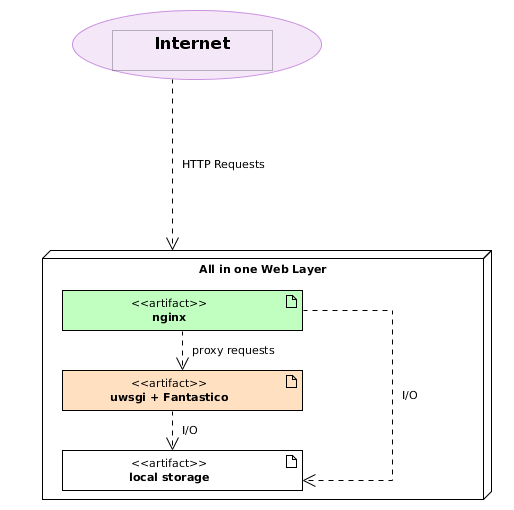
\includegraphics{low_usage_all_in_one.png}

Above diagram described the simplest scenario for rolling out Fantastico to production. You can use this scenario
for minimalistic web applications like:
\begin{itemize}
\item {} 
Presentation website

\item {} 
Personal website

\item {} 
Blog

\end{itemize}

We usually recommend to start with this deployment scenario and the migrate to more complex scenarios when
you application requires it.

\begin{tabulary}{\linewidth}{|L|L|}
\hline
\textbf{\relax 
Advantages
} & \textbf{\relax 
Disadvantages
}\\\hline

Extremely easy to deploy
 & 
Does not scale well for more than couple of requests / second
\\\hline

Minimal os configuration
 & 
All components are bundled on one node without any failover.
\\\hline

Automatic scripts for configuring the os
 & 
Does not support vertical scaling out of the box.
\\\hline

Easy to achieve horizontal scaling for all components at once.
 & 
Static files are not served from a cdn.
\\\hline
\end{tabulary}



\subsubsection{Setup}
\label{how_to/deployment/low_usage_scenario:setup}\begin{enumerate}
\item {} 
Install Fantastico framework on the production machine ({\hyperref[get_started/installation::doc]{\emph{Installation manual}}}.).

\item {} 
Goto \$FANTASTICO\_ROOT/deployment

\item {} 
export ROOT\_PASSWD=\textless{}your root password\textgreater{}

\item {} 
fantastico\_setup\_low\_usage\_\textless{}os\_distribution) --ipaddress \textless{}desired\_ip\textgreater{} --vhost-name \textless{}desired\_vhost\textgreater{} --uwsgi-port \textless{}uwsgi port\textgreater{} --root-folder \textless{}desired root folder\textgreater{} --modules-folder \textless{}desired modules folder\textgreater{} (e.g fantastico\_setup\_low\_usage\_ubuntu.sh --ipaddress 127.0.0.1 --vhost-name fantastico-framework.com --uwsgi-port 12090 --root-folder {}`pwd{}` --modules-folder /fantastico/samples)

\item {} 
Done.

\end{enumerate}

It is usually a good idea to change the number of parallel connections supported by your linux kernel:
\begin{enumerate}
\item {} 
sudo nano /etc/sysctl.conf

\item {} 
Search for \textbf{net.core.somaxconn}.

\item {} 
If it does not exist you can add net.core.somaxconn = 8192 to the bottom of the file.

\item {} 
Restart the os.

\end{enumerate}


\subsection{Low usage AWS}
\label{how_to/deployment/aws_low_usage_scenario:low-usage-aws}\label{how_to/deployment/aws_low_usage_scenario::doc}
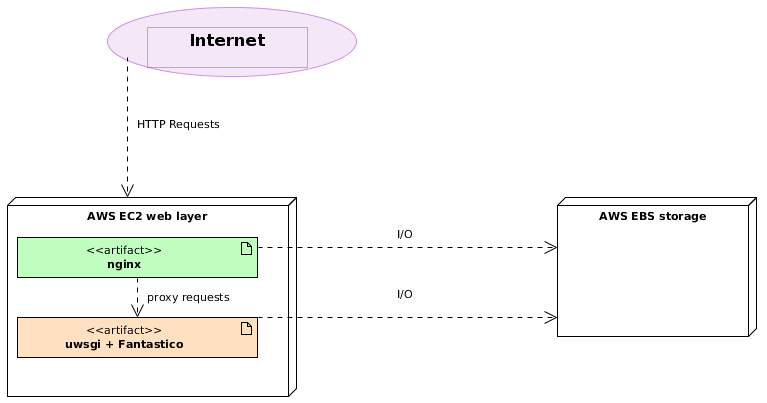
\includegraphics{low_usage_aws.png}

This scenario is a little bit more complex than {\hyperref[how_to/deployment/low_usage_scenario::doc]{\emph{Low usage (simplest scenario)}}} but it provides some
advantages:

\begin{tabulary}{\linewidth}{|L|L|}
\hline
\textbf{\relax 
Advantages
} & \textbf{\relax 
Disadvantages
}\\\hline

Can be autoscaled.
 & 
Requires AWS EC2 instances
\\\hline

Easier crash recovery
 & 
Requires manual configuration
\\\hline

Very easy monitoring support (CloudWatch)
 & 
Requires AWS EBS.
\\\hline
 & 
Requires some AWS know how.
\\\hline
 & 
Static files are not served from a cdn.
\\\hline
\end{tabulary}


This scenario is recommended if you want to rollout you application on AWS infrastructure. Usually it is non expensive
to do this as it requires micro instances and low cost storage. For more information about AWS required components
read:
\begin{enumerate}
\item {} 
\href{http://aws.amazon.com/ec2/instance-types/}{AWS Instance types}.

\item {} 
\href{http://aws.amazon.com/ebs/}{AWS EBS}.

\end{enumerate}


\subsubsection{Setup}
\label{how_to/deployment/aws_low_usage_scenario:setup}\begin{enumerate}
\item {} 
Create an AWS account. (\href{http://aws.amazon.com/documentation/gettingstarted/}{AWS Getting Started}).

\item {} 
Create an EC2 instance from AWS Management Console (\href{http://www.youtube.com/watch?v=WBro0TEAd7g}{EC2 setup}).

\item {} 
SSH on EC2 instance.

\item {} 
Install Fantastico framework on the production machine ({\hyperref[get_started/installation::doc]{\emph{Installation manual}}}.).

\item {} 
Goto \$FANTASTICO\_ROOT/deployment

\item {} 
fantastico\_setup\_low\_usage\_\textless{}os\_distribution).sh (e.g fantastico\_setup\_low\_usage\_ubuntu.sh)

\item {} 
Done.

\end{enumerate}


\subsubsection{Optimization}
\label{how_to/deployment/aws_low_usage_scenario:optimization}
This scenario can be easily optimized by using \textbf{AWS S3} buckets for static files. This ensures faileover for static
files and very easy horizontal scaling for sites. Below you can find the new diagram:

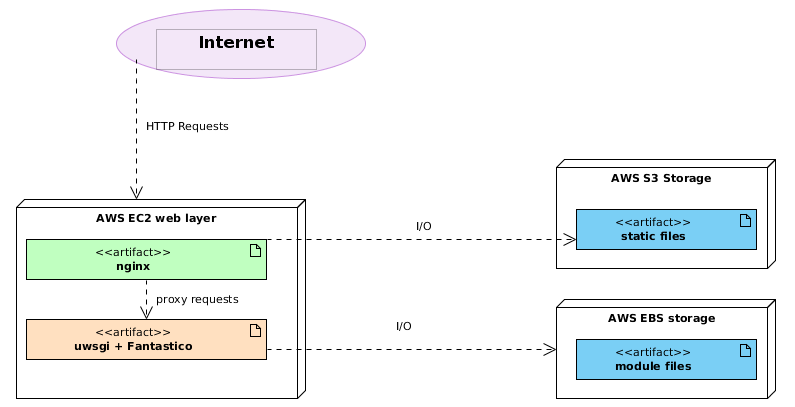
\includegraphics{low_usage_s3_aws.png}

You can read more about \textbf{AWS S3} storage on \href{http://aws.amazon.com/s3/}{http://aws.amazon.com/s3/}. In this version of fantastico there is no
way to sync static module files with S3 buckets. This feature is going to be implemented in upcoming \textbf{Fantastico}
features. As a workaround you can easily copy \textbf{static} folder content from each module on S3 using the tool
provided from AWS Management Console.

You can see how to use AWS Management Console S3 tool on \href{http://www.youtube.com/watch?v=1qrjFb0ZTm8}{http://www.youtube.com/watch?v=1qrjFb0ZTm8}


\subsubsection{Setup with S3}
\label{how_to/deployment/aws_low_usage_scenario:setup-with-s3}\begin{enumerate}
\item {} 
export ROOT\_PASSWD=\textless{}your root password\textgreater{}

\item {} 
Create an AWS account. (\href{http://aws.amazon.com/documentation/gettingstarted/}{AWS Getting Started}).

\item {} 
Create an EC2 instance from AWS Management Console (\href{http://www.youtube.com/watch?v=WBro0TEAd7g}{EC2 setup}).

\item {} 
SSH on EC2 instance.

\item {} 
Install Fantastico framework on the production machine ({\hyperref[get_started/installation::doc]{\emph{Installation manual}}}.).

\item {} 
Goto \$FANTASTICO\_ROOT/deployment

\item {} 
fantastico\_setup\_low\_usage\_s3\_\textless{}os\_distribution).sh --ipaddress \textless{}desired\_ip\textgreater{} --vhost-name \textless{}desired\_vhost\textgreater{} --uwsgi-port \textless{}uwsgi port\textgreater{} --root-folder \textless{}desired root folder\textgreater{} --modules-folder \textless{}desired modules folder\textgreater{} (e.g fantastico\_setup\_low\_usage\_s3\_ubuntu.sh --ipaddress 127.0.0.1 --vhost-name fantastico-framework.com --uwsgi-port 12090 --root-folder {}`pwd{}` --modules-folder /fantastico/samples)

\item {} 
Done.

\end{enumerate}

It is usually a good idea to change the number of parallel connections supported by your linux kernel:
\begin{enumerate}
\item {} 
sudo nano /etc/sysctl.conf

\item {} 
Search for \textbf{net.core.somaxconn}.

\item {} 
If it does not exist you can add net.core.somaxconn = 8192 to the bottom of the file.

\item {} 
Restart the os.

\end{enumerate}


\section{Static assets}
\label{how_to/static_assets:static-assets}\label{how_to/static_assets::doc}
By default, static assets can be any file that is publicly available. Most of the time, here you can place:
\begin{itemize}
\item {} 
css files

\item {} 
png, jpg, gif files

\item {} 
downloadable pdf

\item {} 
movie files

\item {} 
any other file format you can think about

\end{itemize}

For Production environment, requests to these files are handled by the web server you are using. You only need to
place them under \textbf{static} folder of your component ({\hyperref[features/component_model::doc]{\emph{Component model}}}).

There are several scenario in which Fantastico projects are deployed which influence where your component static files
are stored. I recommend you read {\hyperref[how_to/deployment_how_to::doc]{\emph{Deployment how to}}} section.


\subsection{Static assets on dev}
\label{how_to/static_assets:static-assets-on-dev}
Of course, on development environment you are not required to have a web server in front of your Fantastico dev server.
For this purpose, fantastico framework provides a special controller which can easily serve static files. Even though
it works as expected, please do not use it in production. It does not send headers required by browser for caching
purposes.

Static assets routes are the same between \textbf{prod} and \textbf{dev} environments.


\section{Creating a new project}
\label{how_to/new_project_how_to:creating-a-new-project}\label{how_to/new_project_how_to::doc}
A new Fantastico based project can be easily setup by following this how to. In this how to we are going to create
a project named \textbf{fantastico\_first}.
\begin{enumerate}
\item {} 
cd \textasciitilde{}/

\item {} 
mkdir fantastico\_first

\item {} 
cd fantastico\_first

\item {} 
virtualenv-3.2 --distribute pip-deps

\item {} 
. pip-deps/bin/activate

\item {} 
pip install fantastico

\item {} 
fantastico\_setup\_project.sh python3.2 my\_project

\end{enumerate}

The last step might take a while because it will also install all fantastico dependencies (e.g sphinx, sqlalchemy, ...).
Please make sure your replace python3.2 with the correct python version.
In order to test the current project do the following:
\begin{enumerate}
\item {} 
fantastico\_run\_dev\_server

\item {} 
Access \href{http://localhost:12000/fantastico/samples/mvc/static/sample.jpg}{http://localhost:12000/fantastico/samples/mvc/static/sample.jpg}

\item {} 
Access \href{http://localhost:12000/mvc/hello-world}{http://localhost:12000/mvc/hello-world}

\end{enumerate}

Your newly project is setup correctly and it runs fantastico default samples project.


\subsection{Create first component}
\label{how_to/new_project_how_to:create-first-component}
After the new project it's correctly setup we can create our first component.
\begin{enumerate}
\item {} 
. pip-deps/bin/activate

\item {} 
export FANTASTICO\_ACTIVE\_CONFIG=my\_project.settings.BaseProfile

\item {} 
cd my\_project

\item {} 
mkdir component1

\item {} 
cd component1

\item {} 
mkdir static

\item {} 
Paste an image into static folder (e.g first\_photo.jpg)

\item {} 
touch \_\_init\_\_.py

\item {} 
touch hello\_world.py

\item {} 
Paste the code listed below into hello\_world.py

\begin{Verbatim}[commandchars=\\\{\}]
\PYG{k+kn}{from} \PYG{n+nn}{fantastico.mvc.base\PYGZus{}controller} \PYG{k+kn}{import} \PYG{n}{BaseController}
\PYG{k+kn}{from} \PYG{n+nn}{fantastico.mvc.controller\PYGZus{}decorators} \PYG{k+kn}{import} \PYG{n}{ControllerProvider}\PYG{p}{,} \PYG{n}{Controller}
\PYG{k+kn}{from} \PYG{n+nn}{webob.response} \PYG{k+kn}{import} \PYG{n}{Response}

\PYG{n+nd}{@ControllerProvider}\PYG{p}{(}\PYG{p}{)}
\PYG{k}{class} \PYG{n+nc}{HelloWorldController}\PYG{p}{(}\PYG{n}{BaseController}\PYG{p}{)}\PYG{p}{:}
    \PYG{l+s+sd}{\PYGZsq{}\PYGZsq{}\PYGZsq{}This is a very simple controller provider.\PYGZsq{}\PYGZsq{}\PYGZsq{}}

    \PYG{n+nd}{@Controller}\PYG{p}{(}\PYG{n}{url}\PYG{o}{=}\PYG{l+s}{\PYGZdq{}}\PYG{l+s}{/component1/hello}\PYG{l+s}{\PYGZdq{}}\PYG{p}{)}
    \PYG{k}{def} \PYG{n+nf}{say\PYGZus{}hello}\PYG{p}{(}\PYG{n+nb+bp}{self}\PYG{p}{,} \PYG{n}{request}\PYG{p}{)}\PYG{p}{:}
        \PYG{l+s+sd}{\PYGZsq{}\PYGZsq{}\PYGZsq{}This method simply returns an html hello world text.\PYGZsq{}\PYGZsq{}\PYGZsq{}}

        \PYG{n}{msg} \PYG{o}{=} \PYG{l+s}{\PYGZdq{}}\PYG{l+s}{Hello world from my project}\PYG{l+s}{\PYGZdq{}}

        \PYG{k}{return} \PYG{n}{Response}\PYG{p}{(}\PYG{n}{content\PYGZus{}type}\PYG{o}{=}\PYG{l+s}{\PYGZdq{}}\PYG{l+s}{text/html}\PYG{l+s}{\PYGZdq{}}\PYG{p}{,} \PYG{n}{text}\PYG{o}{=}\PYG{n}{msg}\PYG{p}{)}
\end{Verbatim}

\item {} 
fantastico\_dev\_server

\item {} 
Now you can access \href{http://localhost:12000/component1/hello}{Hello route}.

\item {} 
Now you can access \href{http://localhost:12000/component1/static/first\_photo.jpg}{First photo route}.

\end{enumerate}


\subsection{Customize dev server}
\label{how_to/new_project_how_to:customize-dev-server}
For understanding how to customize dev server please read {\hyperref[get_started/dev_mode::doc]{\emph{Development mode}}}


\subsection{Customize uwsgi prod server}
\label{how_to/new_project_how_to:customize-uwsgi-prod-server}
By design, each Fantastico project provides built in support for running it on \href{http://uwsgi-docs.readthedocs.org/en/latest/}{uWSGI server}.
If you want to customize uwsgi parameters for your server you can follow these steps:
\begin{enumerate}
\item {} 
cd \$FANTASTICO\_PROJECT\_FOLDER/deployment/conf/nginx

\item {} 
nano fantastico-uwsgi.ini

\item {} 
Change the options you want and save the file.

\item {} 
fantastico\_run\_prod\_server (for testing the production server).

\item {} 
Be aware that first you need an nginx configured and your project config file deployed (Read {\hyperref[how_to/deployment_how_to::doc]{\emph{Deployment how to}}}).

\end{enumerate}


\chapter{Changes}
\label{changes:changes}\label{changes::doc}\begin{itemize}
\item {} \begin{description}
\item[{v0.1.0}] \leavevmode\begin{itemize}
\item {} 
Built in router that can be easily extended.

\item {} 
WebOb Request / Response architecture.

\item {} 
Request context support for accessing various attributes (current language, current user and other attributes).

\item {} 
Multiple project profiles support.

\item {} 
Database simple configuration for multiple environments.

\item {} 
Model - View - Controller support.

\item {} 
Automatic model facade generator.

\item {} 
Model facade injection into Controllers.

\item {} 
Templating engine support for views (jinja2).

\item {} 
Documentation generator for pdf / html / epub formats.

\item {} 
Automatic framework packaging and deployment.

\item {} 
Helper scripts for creating projects based on Fantastico.

\item {} 
Easy rollout script for running Fantastico projects behind nginx.

\item {} 
Rollout scenarios for deploying Fantastico projects on Amazon (AWS).

\item {} 
How to sections for creating new projects and components using Fantastico.

\end{itemize}

\end{description}

\end{itemize}


\chapter{Build status}
\label{index:build-status}
If you want to see the current build status of the project visit \href{http://jenkins.scrum-expert.ro:8080/job/fantastico-framework/badge/icon/}{Build status}.


\chapter{License}
\label{index:license}
Copyright 2013 Cosnita Radu Viorel

Permission is hereby granted, free of charge, to any person obtaining a copy of this software and associated
documentation files (the ``Software''), to deal in the Software without restriction, including without limitation
the rights to use, copy, modify, merge, publish, distribute, sublicense, and/or sell copies of the Software,
and to permit persons to whom the Software is furnished to do so, subject to the following conditions:

The above copyright notice and this permission notice shall be included in all copies or substantial portions of the Software.

THE SOFTWARE IS PROVIDED ``AS IS'', WITHOUT WARRANTY OF ANY KIND, EXPRESS OR IMPLIED, INCLUDING BUT NOT LIMITED TO THE
WARRANTIES OF MERCHANTABILITY, FITNESS FOR A PARTICULAR PURPOSE AND NONINFRINGEMENT. IN NO EVENT SHALL THE AUTHORS OR
COPYRIGHT HOLDERS BE LIABLE FOR ANY CLAIM, DAMAGES OR OTHER LIABILITY, WHETHER IN AN ACTION OF CONTRACT, TORT OR OTHERWISE,
ARISING FROM, OUT OF OR IN CONNECTION WITH THE SOFTWARE OR THE USE OR OTHER DEALINGS IN THE SOFTWARE.



\renewcommand{\indexname}{Index}
\printindex
\end{document}
